\section{Contribution} \label{contribution}
We propose the \emph{decision design pattern} to detect premature information and present the information maturity-level to a decision-maker. 

\begin{center}
\large\color{document}{The decision design pattern detects incomplete and unreliable information and presents the information maturity-level to a decision-maker.}
\end{center}

We define the reliability of decision-relevant information, described in section \ref{tf_dmm} \nameref{tf_dmm}, using the reproducibility of information, the consensus of evidence, and the conflict of evidence. 

The decision-maker can decide to review the information maturity-level at any moment in time. Some decisions have deadlines, are essential, and potentially have a high impact on an organisation. Decision-makers do not make decisions with a high impact overnight, and they take their time to gather information and understand the exact impact of their decision. The information maturity-level should evolve while the decision-maker adds and changes information and the decision deadline comes closer. This way, the decision-maker uses the transparency of the information maturity-level to increase the completeness and reliability of the decision-relevant information.

\subsection{Decision design pattern}
We bridge the technological knowledge management strategy, described in section \ref{tf-val-rp} \nameref{tf-val-rp}, to the decision design pattern. The evidence-based management pattern stores the knowledge criteria that the decision-makers require to make the decision. The decision ontology pattern uses generic ontology design patterns to define a data structure on top of the evidence-based management pattern. We add the decision presentation pattern to present the information maturity-level. Figure \ref{fig:contribution_architecture} presents the decision design pattern. We encapsulate the completeness, reproducibility, consensus, and conflict patterns into the decision ontology pattern to cover overlap in these patterns and instantiate them in a way they can function side by side.

\begin{figure}[H]
\centering
  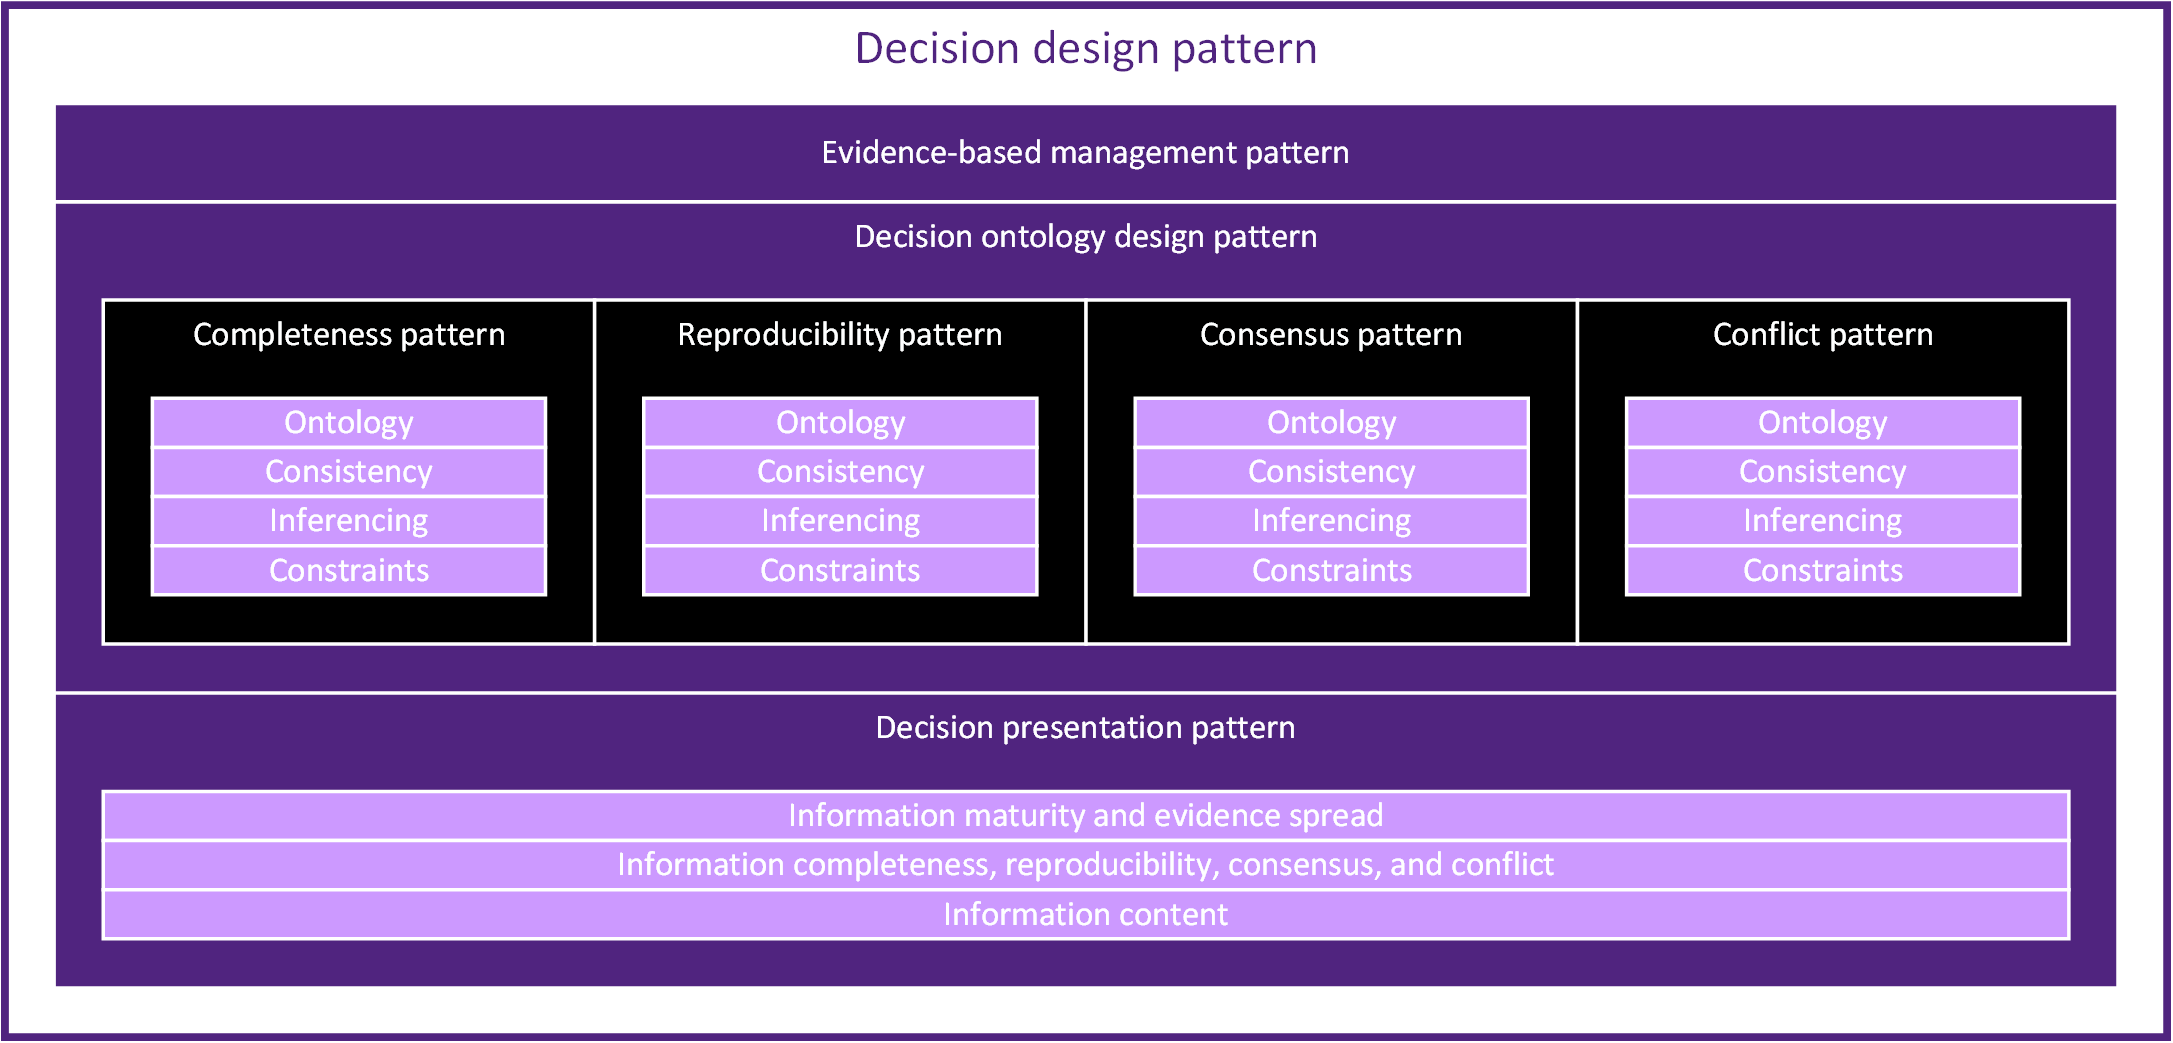
\includegraphics[width=17cm]{../../Images/04_Contribution/Pattern_Architecture.png}
  \caption{An overview of the decision design pattern that detects premature information and presents the information maturity-level. We encapsulate the completeness, reproducibility, consensus, and conflict patterns into the decision ontology design pattern.}
  \label{fig:contribution_architecture}
\end{figure}

We base the information maturity-level on the completeness and reliability of the information. The completeness pattern ensures that the information that a decision-maker needs to make a decision is available. The information needs to be reproducible by relating it to specific evidence sources. Additionally, we use two other patterns to measure the reliability of evidence: the conflict-level, and the consensus-level. The consolidation layer calculates the decision specific information maturity-level. 

With this approach, we deviate slightly from the categories we describe in section \ref{tf_dmm} \nameref{tf_dmm}. We remove the information collection methodology from the scope. We capture a part of the information collection methodology in the evidence types. For example, decision-makers typically gather evidence that we classify as $Contextual\_Circumstance$ using observation while they can only gather $Stakeholder\_Evidence$ by some form of interaction with the stakeholders. 

The decision-maker gets a general understanding of the information completeness and reliability using the information maturity-level and evidence-spread dashboard. We present the completeness, reproducibility, consensus, and conflict maturity-levels when the decision-maker wants to understand the information maturity-level in more details. Last, we present the completeness, reproducibility, consensus, and conflict levels per individual, including the violations. The decision-maker can use these details to increase the information maturity-level of a decision or optimise the evidence-spread. 

We present multiple ontology design patterns in the next sections of this chapter. Each pattern introduces a challenge and the ontology that addresses this challenge. The included generic ontology design pattern enables domain experts to re-use the ontology in different scenarios. Additionally, we describe how we guard the consistency of the ontology, and we describe the inferred information. We present the constraints that detect premature information in the last paragraph. Last, we introduce the main challenge of the decision presentation pattern and describe how we present the information maturity-levels to the decision-maker.

Only the combination of the patterns we describe in this chapter can address the challenge captured by the research question. Therefore, we focus our validation on the combination of patterns in a specific scenario. Section \ref{validation} \nameref{validation} presents the scenario-based validation that combines the patterns into a solution that addresses the challenge of the research question.

\subsection{Evidence-based management pattern} \label{odp_ebm}
% Subsection structure:
% Problem: what is the generalized problem?
% 	Motivation: why is this problem scientifically important and/or interesting?
% Solution: conceptual description of solution, including formal definition of GODP and SHACL constraints.
% 	Illustration: images of GODP structure.
% 	(Statistical)Analysis: how does the solution solve the problem?
% 	Evaluation: are the results significant? What is the impact?
\subsubsection{An evidence-based management structure}
Decision-makers need guidance to make decisions based on reliable information \parencite{DM07}. The evidence-based management pattern provides a structure to store evidence that decision-makers can use as a source for decision-relevant information. The pattern serves as a base for other patterns that validate the information completeness and reliability.

\begin{center}
\large\color{document}{The evidence-based management pattern supports the information completeness and reliability validation patterns by providing an evidence-based management structure.}
\end{center}

\subsubsection{Ontology}
We describe four evidence types in section \ref{tf_dmm} \nameref{tf_dmm}: practitioner expertise and judgement, evaluated external evidence, stakeholder preferences/values, and local context (organisational actors, circumstances). We add the evidence classes $Stakeholder\_Experience$ and $Stakeholder\_Values$ as subclasses of $Stakeholder\_Evidence$. We add $Stakeholder\_Evidence$ as a subclass to $Evidence$ itself. These evidence classes slightly deviate from their original definition. We rename \emph{practitioner} experience to \emph{stakeholder} experience for two reasons:
\begin{enumerate}
\item Practitioners are, generally spoken, a subset of stakeholders: practitioners are also considered stakeholders.
\item The previous definition excluded stakeholder experience and practitioner values as evidence: if stakeholder values are considered evidence, practitioner values should also be considered evidence. This reasoning is also valid for the experience. If we consider practitioner experience as evidence, we should consider stakeholder experience as well. 
\end{enumerate}
We add $Contextual\_Circumstances$ and $Evaluated\_External\_Evidence$ as subclasses of $Evidence$. The reasoner ensures the consistency of the ontology by defining the different evidence classes are disjoint. Figure \ref{fig:classification} presents the structure of the pattern.

\begin{figure}[hbpt]
\centering
  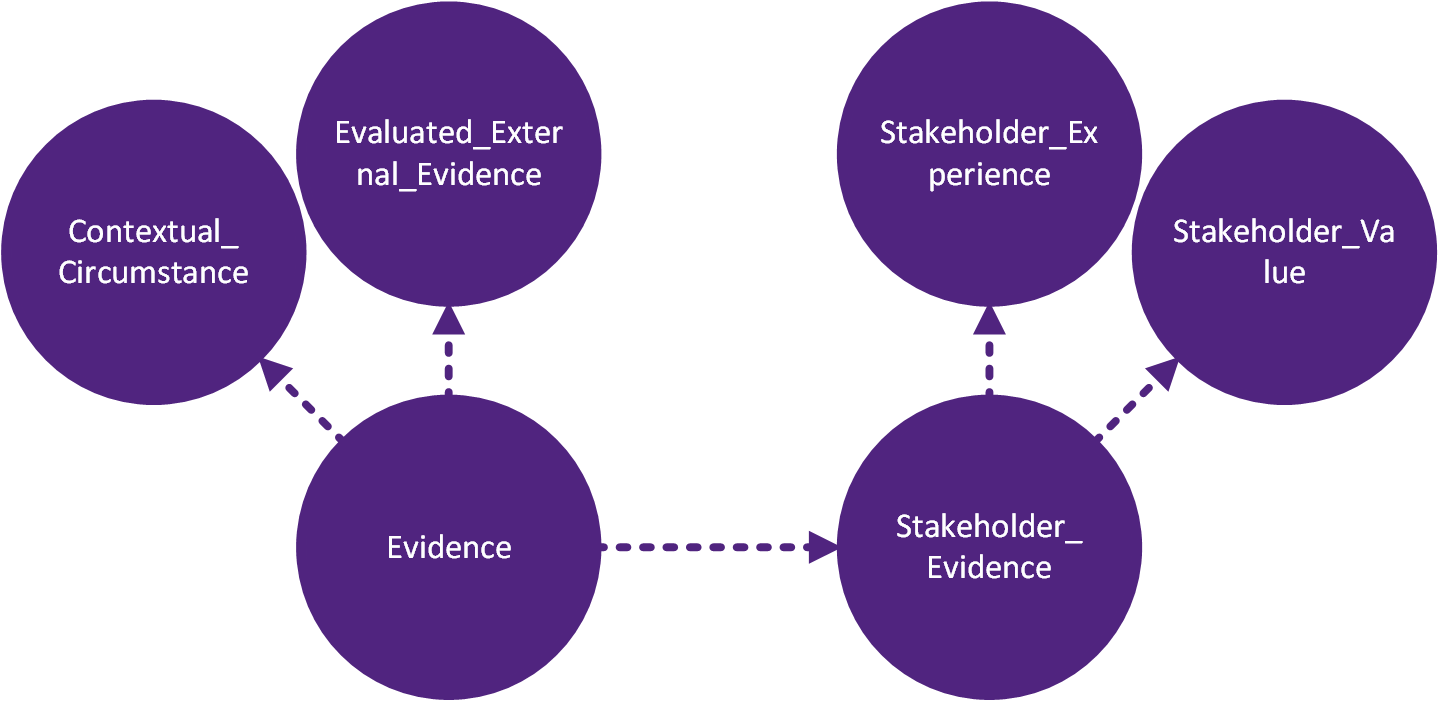
\includegraphics[width=9cm]{../../Images/04_Contribution/04_EBM_Classification.png}
  \caption{An overview of the evidence-based management ontology. $Stakeholder\_Experience$ and $Stakeholder\_Values$ as subclasses of $Stakeholder\_Evidence$. We add $Stakeholder\_Evidence$ as a subclass to $Evidence$ itself. Code sample \ref{GODP_EBM} presents the GDOL code that instantiates this ontology.}
  \label{fig:classification}
\end{figure} 

We create these classes for two purposes. First, the evidence spread determines the reproducibility of the evidence. The decision-maker can decide to gather additional evidence to increase the reproducibility of the decision-relevant information if, for example, the decision-relevant information is only based on $Stakeholder\_Experience$. Second, we extract $Contextual\_Circumstances$ from a written context or observation while we extract $Evaluated\_External\_Evidence$ from other written documents. We can reproduce this evidence based on its source. For $Stakeholder\_Evidence$, we need to know the stakeholder to reproduce it. Different evidence types have different behaviour and, therefore, need different classes.

\paragraph{Consistency}
We guard the consistency of the ontology using $DisjointClasses$. $Stakeholder\_Experience$ is logically different from $Stakeholder\_Value$. An individual cannot be $Stakeholder\_Evidence$, $Contextual\_Circumstance$, or $Evaluated\_External\_Evidence$ at the same time due to the difference in definition. When the reasoner classifies an individual as two disjoint classes, it will throw an inconsistency error and cannot continue reasoning. Figure \ref{fig:consistency_ebm} presents an example of an inconsistency error in Prot\'eg\'e. Code sample \ref{GODP_EBM} presents the implementation of the $DisjointClasses$.

\begin{figure}[H]
\centering
  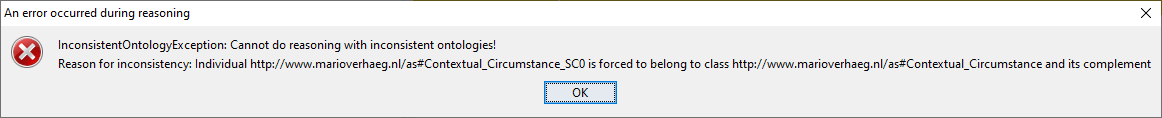
\includegraphics[width=17cm]{../../Images/04_Contribution/Consistency.png}
  \caption{An inconsistent ontology structure that a reasoner detects in Prot\'eg\'e. In this case, the individual $Contextual\_Circumstance\_SC0$ belongs to the classes $Contextual\_Circumstance$ and $Evaluated\_External\_Evidence$. $Contextual\_Circumstance\_SC0$ and $Evaluated\_External\_Evidence$ are disjoint classes. The reasoner does not accept that $Contextual\_Circumstance\_SC0$ belongs to both of these classes.}
  \label{fig:consistency_ebm}
\end{figure}

\paragraph{Inferencing}
The evidence-based management pattern uses a simple structure of classes and does not use inferencing to increase the amount of information in the ontology. 

\paragraph{Generic Ontology Design Pattern}
Code sample \ref{GODP_EBM} presents the generic ontology design pattern of the evidence-based management pattern using GDOL. We instantiate the evidence-based management pattern once per ontology it needs to extend. The evidence-based management pattern does not require parameters; therefore, we instantiate an $ontology$ instead of a $pattern$.

\begin{lstlisting}[float,language=GDOL,caption={The GDOL code that instantiates the generic ontology design pattern for evidence-based management. The instantiation includes the instantiation of the classes as well as the characteristics of those classes. Figure \ref{fig:classification} presents the structure of the pattern. },label={GODP_EBM}][H]
ontology EBM =
 Class: Evidence
 Class: Stakeholder
 Class: Stakeholder_Evidence SubClassOf: Evidence 
 Class: Stakeholder_Experience SubClassOf: Stakeholder_Evidence 
 Class: Stakeholder_Value SubClassOf: Stakeholder_Evidence 
 Class: Contextual_Circumstance SubClassOf: Evidence 
 Class: Evaluated_External_Evidence SubClassOf: Evidence 
 DisjointClasses: Stakeholder_Evidence, Contextual_Circumstance, Evaluated_External_Evidence	
 DisjointClasses: Stakeholder_Experience, Stakeholder_Value
\end{lstlisting}

\paragraph{Constraints}
It is possible to define constraints based on the stake of a specific evidence type. For example, the $Evaluated\_External\_Evidence$ should represent 20\% of the evidence related to a specific decision. However, these constraints would be very context-sensitive. We leave it up to the decision-maker to evaluate the mix of evidence-types manually on a case-by-case basis. Alternatively, the domain expert can manually add constraints based on the preference of the organisation implementing the decision design pattern. 
\subsection{Decision ontology pattern} \label{odp_decision_ontology}
% Subsection structure:
% Problem: what is the generalized problem?
% 	Motivation: why is this problem scientifically important and/or interesting?
% Solution: conceptual description of solution, including formal definition of GODP and SHACL shapes.
% 	Illustration: images of GODP structure.
% 	(Statistical)Analysis: how does the solution solve the problem?
% 	Evaluation: are the results significant? What is the impact?
\subsubsection{An information maturity-level structure}
The evidence-based management, completeness, reproducibility, consensus, and conflict patterns solve separate generic problems. At the same time, these patterns overlap in their ontology structure. This overlap makes it difficult to use these patterns in the same environment. The decision design pattern provides the glue between the completeness, reproducibility, consensus, and conflict patterns, using the evidence-based management pattern as a base. 

The decision presentation pattern combines the output from the completeness, reproducibility, consensus, and conflict patterns to calculate the \emph{information maturity-level} for a decision. The decision-maker needs to make a \emph{meta-decision} based on the information maturity-level:
\begin{enumerate}
\item If the information maturity-level is acceptable, the decision-maker can make the main-decision.
\item If the information maturity-level is not acceptable, the decision-maker needs to increase the information maturity-level until it is acceptable.
\end{enumerate}

The outcome of the meta-decision depends on the complexity and impact of the main-decision. If the complexity and impact of the main-decision are low, a lower information maturity-level might be acceptable. However, if the impact and complexity of the main-decision are high, we expect that the requirements towards the information maturity-level are higher as well. 

\begin{center}
\large\color{document}{The decision ontology pattern increases the transparency of the completeness and reliability of decision-relevant information.} 
\end{center}

The scale of the impact and complexity of a decision are organisation dependent. For example, a C-level decision in an organisation with 3000 employees has a different impact compared to a C-level decision in an organisation with 300 employees. As a result, we cannot automate this meta-decision. In essence, a human needs to evaluate, based on knowledge and experience, if the complexity and impact of the decision justify the information maturity-level.

\subsubsection{Completeness} \label{odp_completeness}
% Subsection structure:
% Problem: what is the generalized problem?
% 	Motivation: why is this problem scientifically important and/or interesting?
% Solution: conceptual description of solution, including formal definition of GODP and SHACL shapes.
% 	Illustration: images of GODP structure.
% 	(Statistical)Analysis: how does the solution solve the problem?
% 	Evaluation: are the results significant? What is the impact?
\paragraph{Detecting completeness}
A decision-maker makes a decision knowing context-relevant information for that specific decision. Some information crucial for decision $x$ might be irrelevant for decision $y$. Each decision requires different context-relevant information. This pattern allows a domain expert to define the context-relevant information.

\begin{center}
\large\color{document}{The completeness pattern validates the completeness of information by detecting missing information.}
\end{center}

\paragraph{Ontology}
The completeness pattern detects if an individual classified as $C$ is incomplete, considering a required property $p$. We achieve this by creating a data property or an object property and use parameters to define its domain and range. The constraints detect individuals classified as $C$ that do not host the data or object property. The detected individuals are considered incomplete and, therefore, premature.

\paragraph{Inferencing}
The completeness pattern infers the class of individuals from the domain or range of the data or object property. For example, if $Information$ is the domain of the property $data\_description$, then the reasoner will infer individuals that have a $data\_description$ as $Information$. Figure \ref{fig:04_data_description} presents this example in Prot\'eg\'e.

\begin{figure}[H]
\centering
  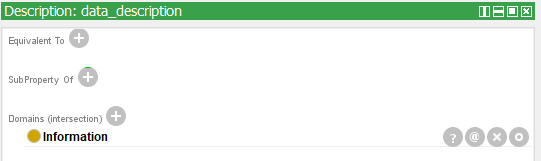
\includegraphics[width=10cm]{../../Images/04_Contribution/04_data_description.png}
  \caption{If $Information$ is the domain of the property $data\_description$, then the reasoner will infer individuals that have a $data\_description$ as $Information$.}
  \label{fig:04_data_description}
\end{figure}

\paragraph{Inconsistency}
Code sample \ref{GODP_COMP} presents the generic ontology design pattern to create a data property. This code sample includes a range. The definition of the range limits the data range that the data property accepts, for example, a $xsd:string$ accepts strings or $xsd:int$ accepts integers. The ontology is inconsistent when the data property stores a value that is outside of the defined range.

\paragraph{Generic ontology design pattern}
Code sample \ref{GODP_COMP} adds a data property or an object property to an existing class. We use three parameters to instantiate the data or object property: $c$ defines the class that should host the data property, $p$ defines the data property itself, and $r$ defines the range of the data property. We use the range of the data property to restrict its content using, for example, regular expressions and use the range of the object property to infer the class of an individual. Figure \ref{fig:GODP_COMP_DP} presents the data property, and figure \ref{fig:GODP_COM_OP} presents the object property.

\begin{lstlisting}[float,language=GDOL,caption={The GDOL code for adding a required data property to an existing class using two parameters. We use $c$, $i$, and $r$ as parameters to instantiate the data or object property.},label={GODP_COMP}][H]
pattern Completeness_dp [Class: c; DataProperty: i; Datatype: r] =
	DataProperty: i Domain: c Range: r
pattern Completeness_op [Class: c; ObjectProperty: i; Datatype: r] =
	ObjectProperty: i Domain: c Range: r
\end{lstlisting}

\begin{figure}[H]
\centering
  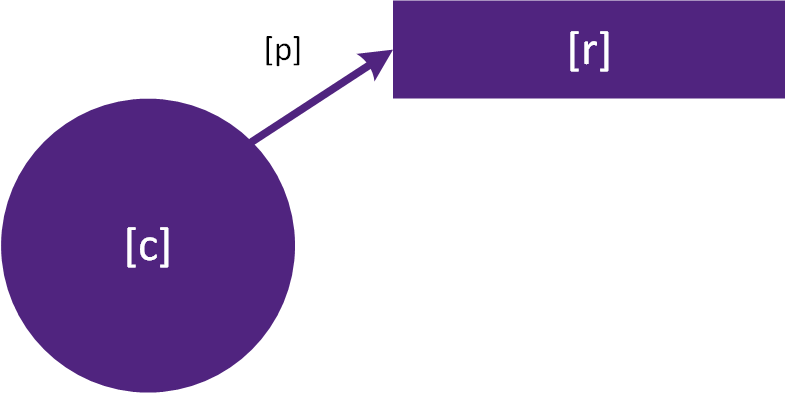
\includegraphics[width=5cm]{../../Images/04_Contribution/Completeness_DP.png}
  \caption{The completeness of a class using a data property. Code sample \ref{GODP_COMP} presents the GDOL code for adding a data property to an existing class. Code sample \ref{GODP_COMP} presents the GDOL code that instantiates this ontology.}
  \label{fig:GODP_COMP_DP}
\end{figure} 

\begin{figure}[H]
\centering
  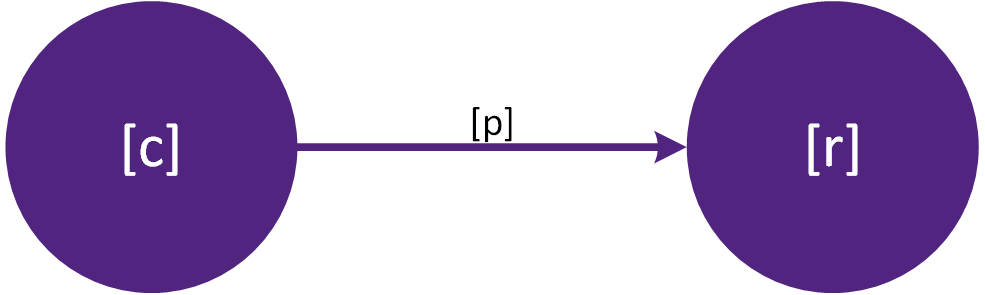
\includegraphics[width=6cm]{../../Images/04_Contribution/Completeness_OP.png}
  \caption{The completeness of a class using an object property. Code sample \ref{GODP_COMP} presents the GDOL code for adding an object property to an existing class. Code sample \ref{GODP_COMP} presents the GDOL code that instantiates this ontology.}
  \label{fig:GODP_COM_OP}
\end{figure} 

\paragraph{Constraints}
The SHACL shape in code sample \ref{SHACL_COM_DP} detects when an individual classified as $c$ does not host the defined data or object property $p$. Each individual classified as $c$ should have at least one path (object or data property) $p$. The SHACL shape monitors the existence of the data or object property using the cardinality constraint $minCount$. $c$ and $p$ set the context of the constraints.

\begin{lstlisting}[float,language=SHACL,caption={The SHACL code that validates if the individuals classified as $c$ host the property $p$. We use the cardinality constraint $sh:minCount$ for this detection: each individual classified as $c$ should have at least one path (object or data property) $p$.},label={SHACL_COM_DP}][H]
[c]Shape a sh:NodeShape;
	sh:targetClass [c]; 
	sh:property [
		sh:path [p]; 
		sh:severity sh:Violation; 
		sh:minCount 1; 
		sh:message "Completeness: add [c] to [p]."; ]
\end{lstlisting} 
\subsubsection{Reproducibility} \label{odp_reproducibility}
% Subsection structure:
% Problem: what is the generalized problem?
% 	Motivation: why is this problem scientifically important and/or interesting?
% Solution: conceptual description of solution, including formal definition of GODP and SHACL shapes.
% 	Illustration: images of GODP structure.
% 	(Statistical)Analysis: how does the solution solve the problem?
% 	Evaluation: are the results significant? What is the impact?
\paragraph{Detecting reproducibility}
We use reproducibility to evaluate the reliability of decision-relevant information. The reproducibility pattern can detect when information cannot be traced back to an evidence source. When evidence cannot be traced back to an evidence source, the pattern detects the information as premature. 

\begin{center}
\large\color{document}{The reproducibility pattern validates the information reliability by detecting when information cannot be traced back to an evidence source.}
\end{center}

\paragraph{Ontology}
Information is reproducible when it can be traced back to evidence or an information source, for example, a contextual circumstance or the value of a stakeholder. This pattern relates information to an evidence source using an object property. An information class can be based on another information class as well, as long as the chain of information is evidence-based. We use the completeness pattern to ensure the required data properties are available. Figure \ref{fig:reproducibility_chain} presents a chain that connects information to evidence. The $based\_on\_in{\f}ormation$ object property is transitive. When we base information $a$ on information $b$, and information $b$ on information $c$, then information $a$ is also based on information $c$. We need the transitive characteristic to query the evidence sources of information for the decision presentation pattern.

\begin{figure}[H]
\centering
  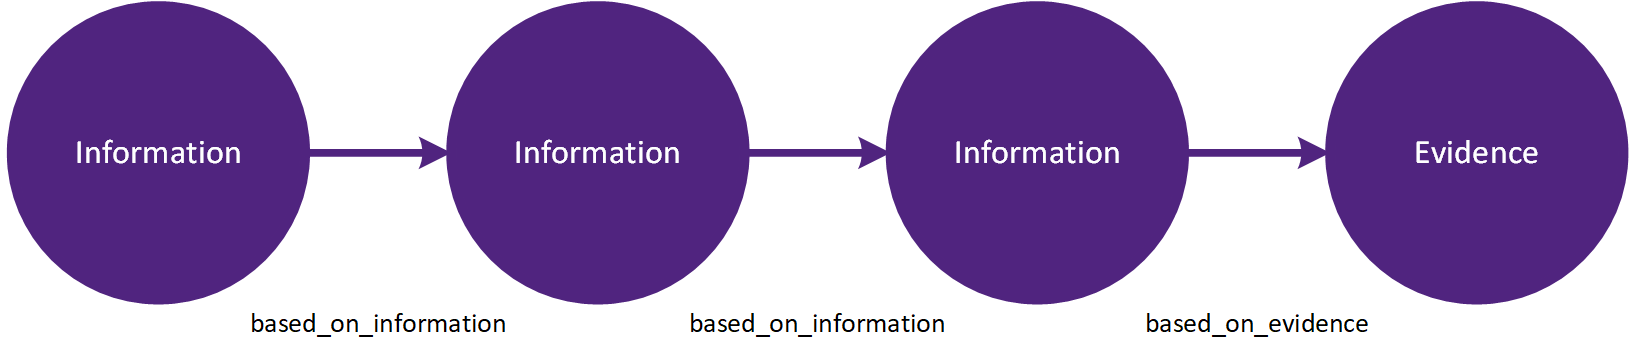
\includegraphics[width=13cm]{../../Images/Reproducibility_Chain.png}
  \caption{An example of an evidence-based chain of information. The reproducibility pattern should detect if the information in the chain is not evidence-based.}
  \label{fig:reproducibility_chain}
\end{figure} 

We extend the evidence-based management pattern in two ways:
\begin{enumerate}
\item Contextual circumstances and evaluated external evidence naturally refer to their actual evidence source, for example, a scientific article or an observation. Stakeholder evidence requires a specific stakeholder as a source of evidence. We extend the evidence-based management pattern with one class ($Stakeholder$) and the related object property ($shared\_by$). 
\item Individuals (classified as $In{\f}ormation$) hosting data properties should be evidence-based or information-based. The object property $based\_on\_evidence$ relates a class to the evidence class. The object property $based\_on\_in{\f}ormation$ relates a class to an information class. 
\end{enumerate} 

Figure \ref{fig:reproducibility} presents the resulting ontology. We have marked the extensions of the evidence-based management pattern in \textcolor{DarkBlue}{blue}.

\begin{figure}[H]
\centering
  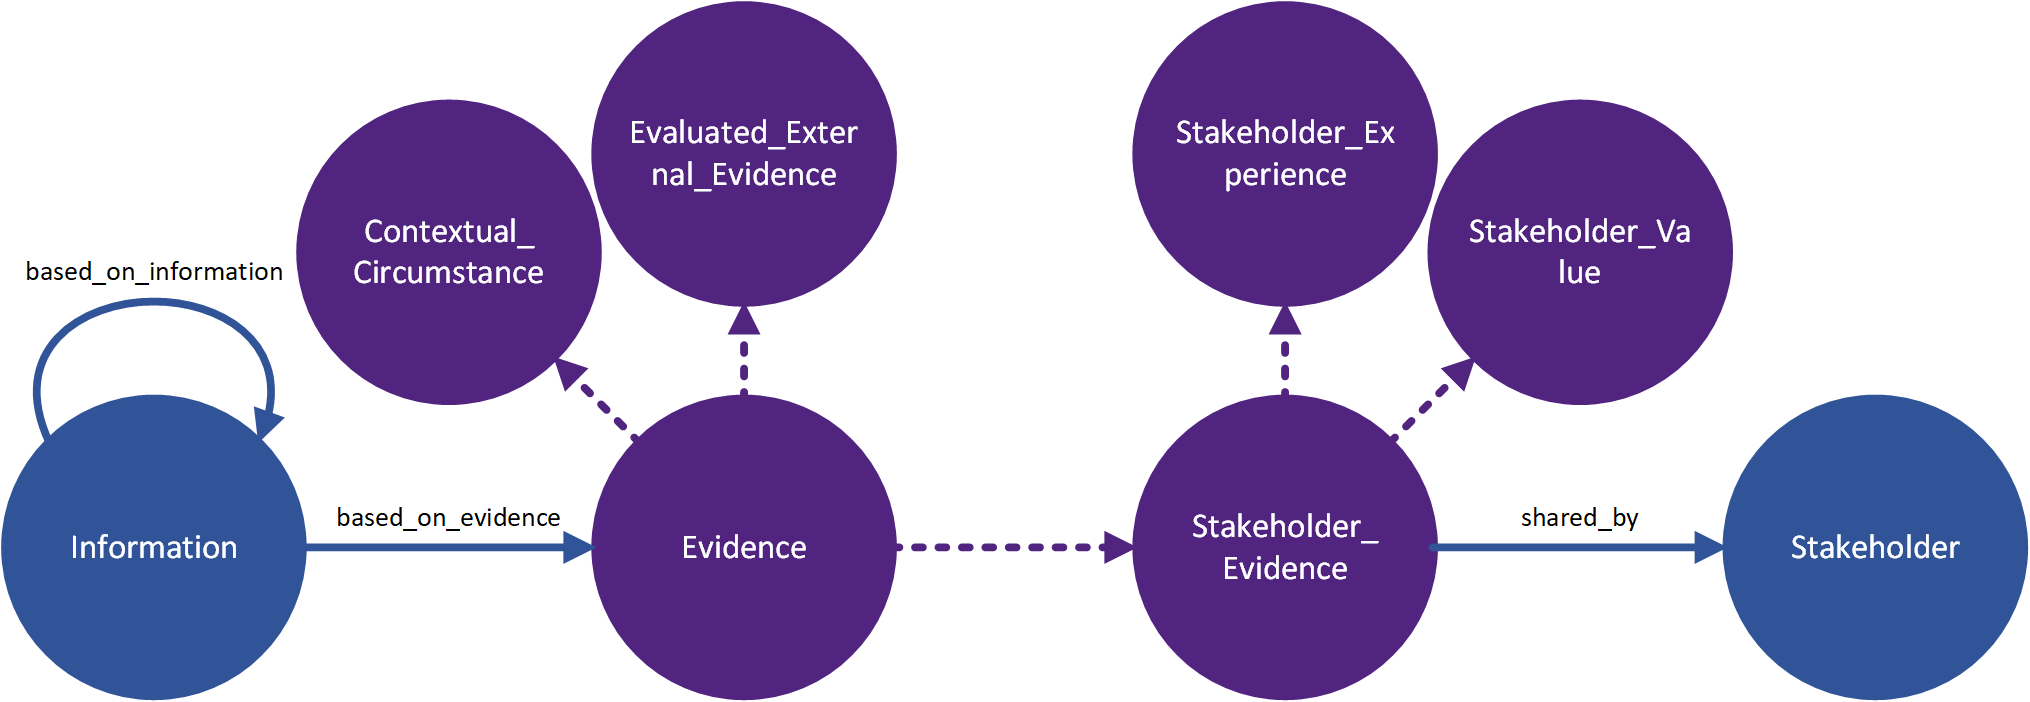
\includegraphics[width=14cm]{../../Images/04_Contribution/04_Reproducibility_Ontology.png}
  \caption{The reproducibility ontology. We have marked the extensions of the evidence-based management pattern in \textcolor{DarkBlue}{blue}. Code sample \ref{GODP_REP_EXT} presents the GDOL code that we use to instantiate this pattern.}
  \label{fig:reproducibility}
\end{figure}

\paragraph{Inferencing}
We use the domain and range of the $based\_on\_information$, $based\_on\_evidence$, and $shared\_by$ object properties to allow the reasoner to classify individuals that are using these object properties. Table \ref{table:rep_inference} presents the classification the reasoner infers from the domain and range configuration.

\begin{table}[H]
\centering
\caption{We use the domain and range of the $based\_on\_in{\f}ormation$, $based\_on\_evidence$, and $shared\_by$ object properties to allow the reasoner to classify individuals that are using these object properties.}
\begin{tabular}{| p{4cm} | p{6cm} |  p{4cm} |   }
\hline
\rowcolor{document}
\color{documentText}Domain & \color{documentText}Object property & \color{documentText}Range \\
\hline
$In{\f}ormation$ & $based\_on\_in{\f}ormation$ & $In{\f}ormation$ \\
\hdashline
$In{\f}ormation$ & $based\_on\_evidence$ & $Evidence$ \\
\hdashline
$Stakeholder\_Evidence$ & $shared\_by$ & $Stakeholder$ \\
\hline
\end{tabular}
\label{table:rep_inference}
\end{table}

\paragraph{Inconsistency} \label{rep_incons}
We guard the consistency of the ontology using $DisjointClasses$. The reasoner cannot classify an individual as $Information$ and $Evidence$ at the same time. If we allow the reasoner to do this, it might create a circular dependency in the reproducibility chain figure \ref{fig:reproducibility_chain} presents. $In{\f}ormation$ typically represents a statement that we can trace back to at least one $Evidence$ source. Code sample \ref{GODP_REP_EXT} presents the implementation of the $DisjointClasses$.

\paragraph{Generic ontology design pattern}
Figure \ref{fig:reproducibility} presents an ontology that extends the evidence-based management ontology and enables the detection of unreproducible information. Code sample \ref{GODP_REP_EXT} presents the GDOL code that extends the evidence-based management ontology. 

\begin{lstlisting}[float,language=GDOL,caption={The GDOL code for relating information to evidence and stakeholder evidence to a stakeholder. We introduce two new classes ($Stakeholder$ and $Information$) and three new object properties ($shared\_by$, $based\_on\_evidence$, and $based\_on\_in{\f}ormation$. Additionally, we define that $Information$ and $Evidence$ are disjoint. Figure \ref{fig:reproducibility} visualises the result of executing the code.},label={GODP_REP_EXT}][H]
ontology Reproducibility_Basic = EBM then 
 Class: Stakeholder 
 Class: Information 
 ObjectProperty shared_by Domain: Stakeholder_Evidence Range: Stakeholder 
 ObjectProperty based_on_evidence Domain: Information Range: Evidence
 ObjectProperty based_on_information Domain: Information Range: Information Characteristics: Transitive
 DisjointClasses: Information, Evidence
\end{lstlisting}

The classes that store decision-relevant information are required to be a subclass of $In{\f}ormation$. Code sample \ref{GODP_REP_EV} presents the GDOL code that relates information to evidence. The inferencing using the domain and range of the $based\_on\_in{\f}ormation$, $based\_on\_evidence$, and $shared\_by$ object properties contributes to this classification as well.

\begin{lstlisting}[float,language=GDOL,caption={The GDOL code that classifies individuals as a sub-class of $Information$. We use $dri$ (decision relevant information) and $i$ (information) as parameters.},label={GODP_REP_EV}][H]
pattern Reproducibility_Context [Class: dri; Class: i] = 
 Class: [dri] SubClassOf: [i]
\end{lstlisting}

\paragraph{Constraints}
Code sample \ref{SHACL_REP} presents the SHACL shape that detects unreproducible information. Each individual that is classified as $In{\f}ormation$ is required to host the object property $based\_on\_in{\f}ormation$ or $based\_on\_evidence$. Individuals that are classified as $In{\f}ormation$ can be traced back to an evidence or information source by hosting one of these two object properties. If the individual does not host one of the object properties, its information cannot be traced back to an evidence source, and the pattern detects the information as premature. The SHACL shape monitors the existence of the object properties using the cardinality constraint $minCount$. 

\begin{lstlisting}[float,language=SHACL,caption={The SHACL code that detects if $Information$ is not $based\_on\_evidence$ or $based\_on\_in{\f}ormation$. The SHACL shape monitors the existence of these object properties using the cardinality constraint $minCount$. },label={SHACL_REP}][H]
Used_InformationShape a sh:NodeShape;
	sh:targetClass Information; 
	sh:property [
		sh:or (
			[sh:path based_on_information; sh:minCount 1;]
			[sh:path based_on_evidence; sh:minCount 1;]
		)
		sh:severity sh:Violation; 
		sh:message "Reproducibility: enter an information or evidence source for this information."; ];
\end{lstlisting}

Code sample \ref{SHACL_REP_SH} presents the SHACL shape that detects when the pattern cannot trace back $Stakeholder\_Experience$ or a $Stakeholder\_Value$ to a $Stakeholder$. We use the $shared\_by$ combined with the cardinality constraints $sh:minCount$ object property to achieve this. The constraints generate a violation if an individual that is classified as $Stakeholder\_Evidence$ is not $shared\_by$ a stakeholder.

\begin{lstlisting}[float,language=SHACL,caption={The SHACL code that detects when a stakeholder does not share $Stakeholder\_Evidence$. We use the cardinality constraint $sh:minCount$ for this detection: each individual classified as $Stakeholder\_Evidence$ should have at least one path $shared\_by$. The range of $shared\_by$ is $Stakeholder$.},label={SHACL_REP_SH}][H]
StakeholderShape a sh:NodeShape;
	sh:targetClass Stakeholder_Evidence; 
	sh:property [
		sh:path shared_by;
		sh:severity sh:Violation; 
		sh:minCount 1; 
		sh:message "Reproducibility: enter a stakeholder that serves as the source of this stakeholder evidence."; ];
\end{lstlisting} 
\subsubsection{Consensus} \label{odp_consensus}
% Subsection structure:
% Problem: what is the generalized problem?
% 	Motivation: why is this problem scientifically important and/or interesting?
% Solution: conceptual description of solution, including formal definition of GODP and SHACL shapes.
% 	Illustration: images of GODP structure.
% 	(Statistical)Analysis: how does the solution solve the problem?
% 	Evaluation: are the results significant? What is the impact?
\paragraph{Detecting consensus}
Information that is based on multiple evidence sources is more reliable than information that is based on one evidence source. For example, one scientific paper supported by stakeholder experience is more reliable than a scientific paper alone. 

\begin{center}
\large\color{document}{The consensus pattern validates the evidence reliability by detecting when evidence does not agree with at least one additional evidence source.}
\end{center}

\paragraph{Ontology}
We define consent evidence as evidence that agrees with at least one other evidence source. The reproducibility pattern provides the structure on which we create the consensus pattern. We introduce the $agrees\_with$ object property. Figure \ref{fig:consensus} presents the consensus pattern. We mark the extension of the reproducibility pattern in \textcolor{LightGreen}{green}. For example, if two stakeholders have the same experience, the $agrees\_with$ object property can link this stakeholder experience. 

\begin{figure}[H]
\centering
  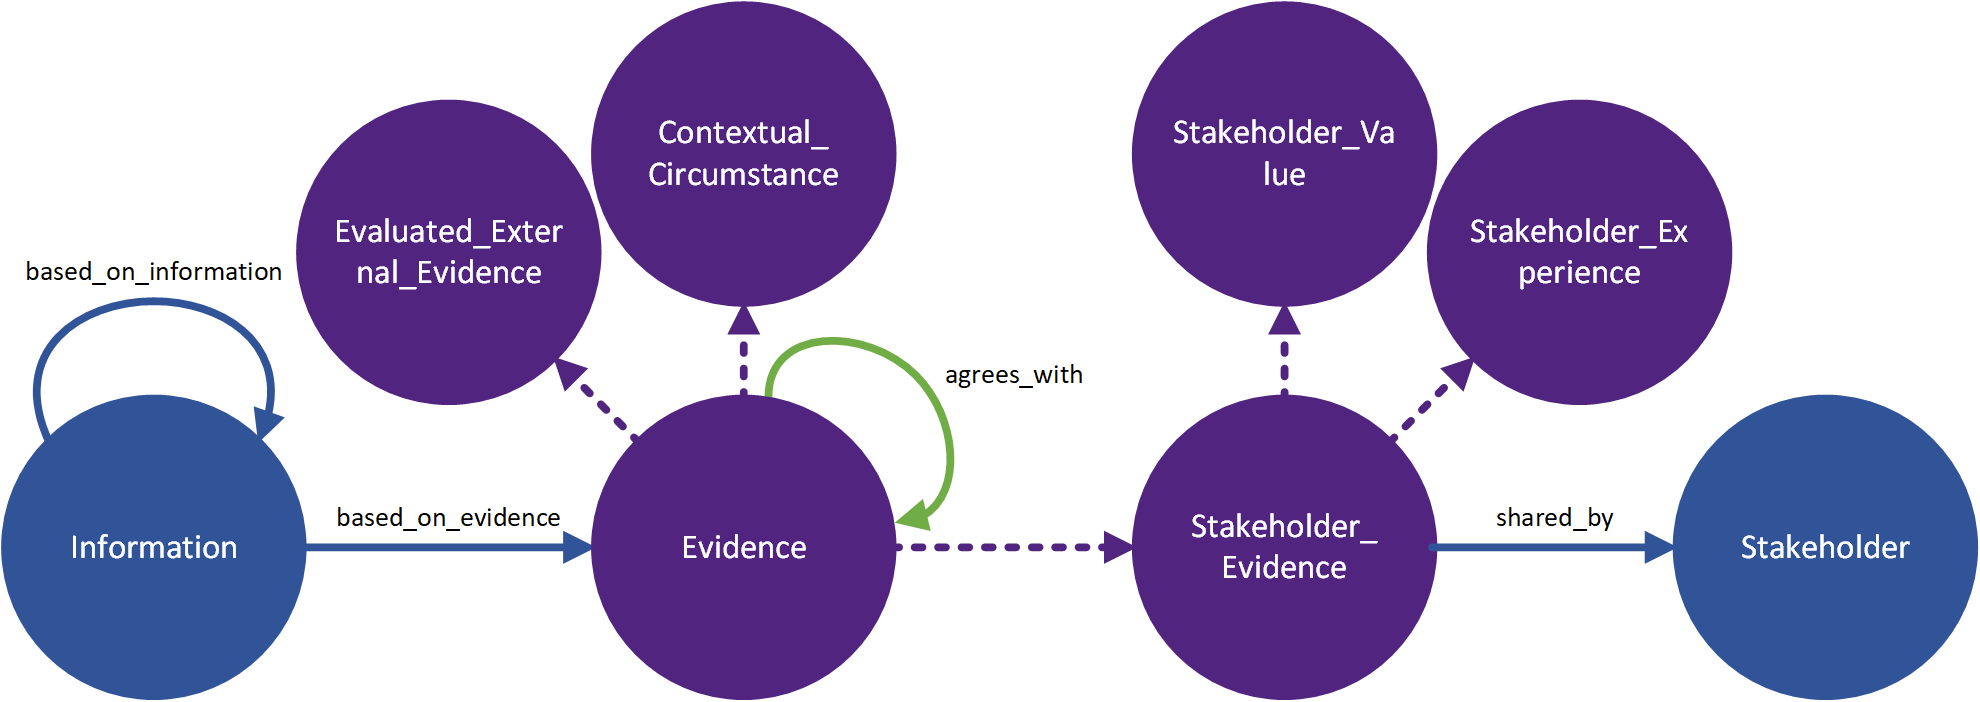
\includegraphics[width=14cm]{../../Images/04_Contribution/04_Consensus_Ontology.png}
  \caption{The consensus pattern that we have based on the reproducibility pattern. We have extended the reproducibility pattern with the object property $agrees\_with$. Code sample \ref{GODP_CON_LEV} extends the reproducibility pattern using GDOL.}
  \label{fig:consensus}
\end{figure}

\paragraph{Inferencing}
We can measure the consensus-level of an evidence source using the $agrees\_with$ object property. We extend the $based\_on\_evidence$ object property with a super property. When we base $In{\f}ormationX$ on $EvidenceA$, and $EvidenceA$ agrees with $EvidenceB$, the reasoner bases $In{\f}ormationX$ on $EvidenceB$ as well. Figure \ref{fig:consensus_inferred} presents the super property that infers this knowledge from the existing ontology structure.

\begin{figure}[H]
\centering
  
\includegraphics[width=17cm]{../../Images/Consensus_Inferred.png}
  \caption{The super property that infers the object property $based\_on\_evidence$ in Prot\'eg\'e.}
  \label{fig:consensus_inferred}
\end{figure}

The $agrees\_with$ object property is symmetric. If individual $A$ agrees with individual $B$, individual $B$ should also agree with individual $A$. Figure \ref{fig:consensus_transitive} presents the characteristics of the $agrees\_with$ object property.

\begin{figure}[H]
\centering
  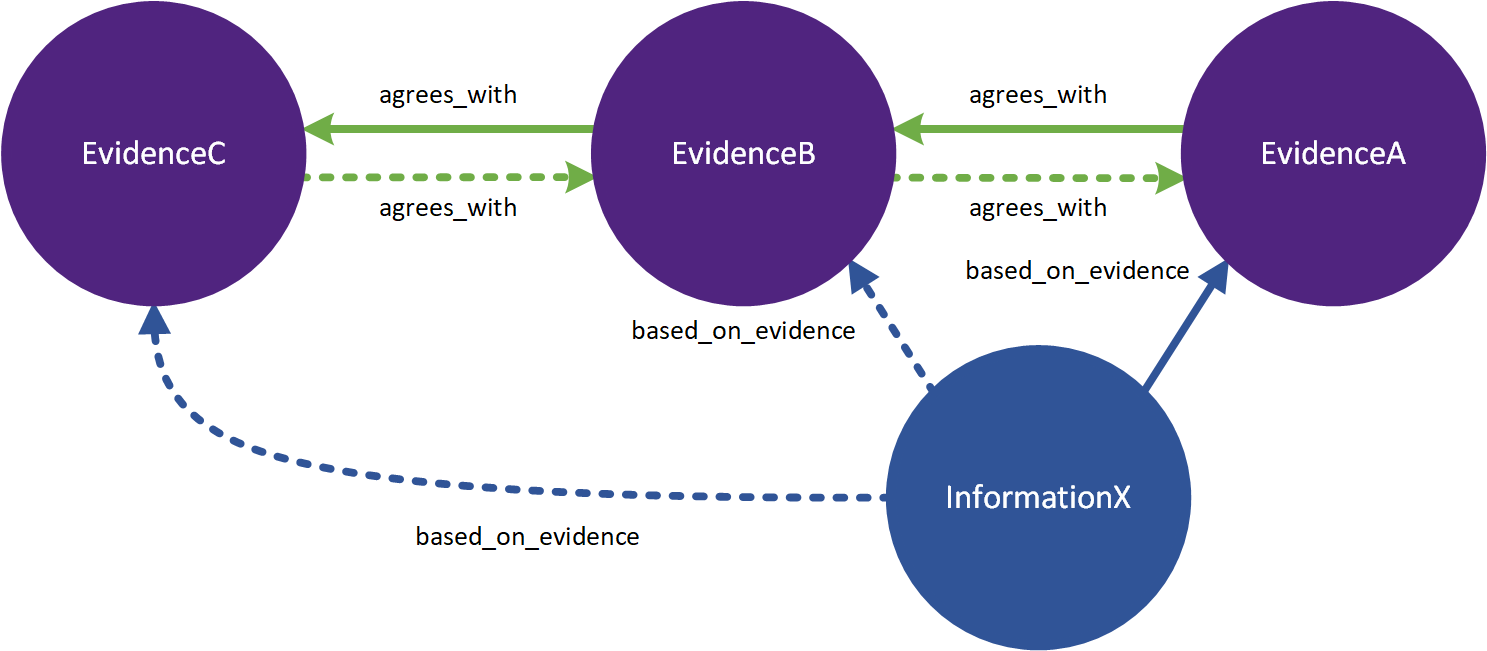
\includegraphics[width=13cm]{../../Images/04_Contribution/04_Consensus_Characteristics.png}
  \caption{An example of the impact of the symmetric characteristics of the $agrees\_with$ object property. The reasoner infers the dotted lines based on the super property figure \ref{fig:consensus_inferred} presents and the symmetric characteristics of $agrees\_with$.}
  \label{fig:consensus_transitive}
\end{figure}

\paragraph{Inconsistency}
The consensus pattern inherits the consistency validation from the reproducibility pattern. We describe the consistency of the reproducibility pattern in section \ref{rep_incons} \nameref{rep_incons}.

\paragraph{Generic ontology design pattern}
Code sample \ref{GODP_CON_LEV} presents the described solution into GDOL. We take the $Reproducibility\_Basic$ pattern, introduce the $agrees\_with$ object property, and extend the $based\_on\_evidence$ object property. 

\begin{lstlisting}[float,language=GDOL,caption={The GDOL code that extends the reproducibility pattern and results in the consensus pattern. We take the $Reproducibility\_Basic$ pattern, introduce the $agrees\_with$ object property, and extend the $based\_on\_evidence$ object property. Figure \ref{fig:consensus} presents the generic ontology design pattern.},label={GODP_CON_LEV}][H]
ontology Consensus = Reproducibility_Basic then
 ObjectProperty: agrees_with Domain: Evidence Range: Evidence Characteristics: Symmetric
 ObjectProperty: based_on_evidence SubPropertyChain: based_on_evidence o agrees_with SubPropertyOf: based_on_evidence
\end{lstlisting}

\paragraph{Constraints}
We define one consensus level for each individual classified as $Evidence$. We set the consensus-level to $1$. This consensus level ensures that each used evidence source has at least one other agreeable evidence source. The minimum consensus level can be adjusted depending on the environment. For example, in life-safety environments, the consensus level might be increased. We use the cardinality constraint $sh:minCount$ for the consensus detection: each individual classified as $Evidence$ should have at least one path $agrees\_with$.

\begin{lstlisting}[float,language=SHACL,caption={The SHACL shapes that detect when information does not meet the minimum consensus level.},label={SHACL_CON_LEV}][H]
UsedEvidenceShape a sh:NodeShape;
	sh:targetClass Evidence; 
	sh:property [
		sh:path agrees_with; 
		sh:severity sh:Violation; 
		sh:minCount 1; 
		sh:message "Consensus: ensure the evidence is in agreement with at least one additional evidence source."; ];
\end{lstlisting} 
\subsubsection{Conflict} \label{odp_conflict}
% Subsection structure:
% Problem: what is the generalized problem?
% 	Motivation: why is this problem scientifically important and/or interesting?
% Solution: conceptual description of solution, including formal definition of GODP and SHACL shapes.
% 	Illustration: images of GODP structure.
% 	(Statistical)Analysis: how does the solution solve the problem?
% 	Evaluation: are the results significant? What is the impact?
\paragraph{Detecting conflict}
Information that has conflicting evidence sources is less reliable compared to information that does not have conflicting evidence sources. For example, stakeholder experience that is conflicting with evaluated external evidence is less reliable compared to stakeholder experience that does not have any conflict. We define the number of evidence sources that causes a conflict with the decision-relevant information as the level of conflict. We define the level of conflict using the reproducibility of information. When information is reproducible by one evidence source, and this evidence source has one additional conflicting evidence source, the level of conflict is $1$. When the evidence source has two conflicting evidence sources, the level of conflict is $2$. Compared to a fuzzy approach that can classify certain conflict levels as, for example, $low$, $medium$, or $high$, the number-based approach makes it easier to compare conflict levels. We do not compare conflict-levels in this study.

\begin{center}
\large\color{document}{The conflict pattern validates information reliability by detecting conflicting evidence.} 
\end{center}

\paragraph{Ontology}
We define conflicting evidence as evidence that disagrees with another evidence source. The reproducibility pattern serves as a natural base for the conflict pattern. The reproducibility pattern provides the structure on which we create the conflict pattern using the object property $disagrees\_with$. Figure \ref{fig:conflict} presents the conflict pattern. We mark the extension of the conflict pattern in \textcolor{Red}{red}. We measure the level of conflict between evidence sources using the $disagrees\_with$ object property. For example, if two stakeholders have a different experience, the $disagrees\_with$ object property represents this conflicting stakeholder experience. 

\begin{figure}[H]
\centering
  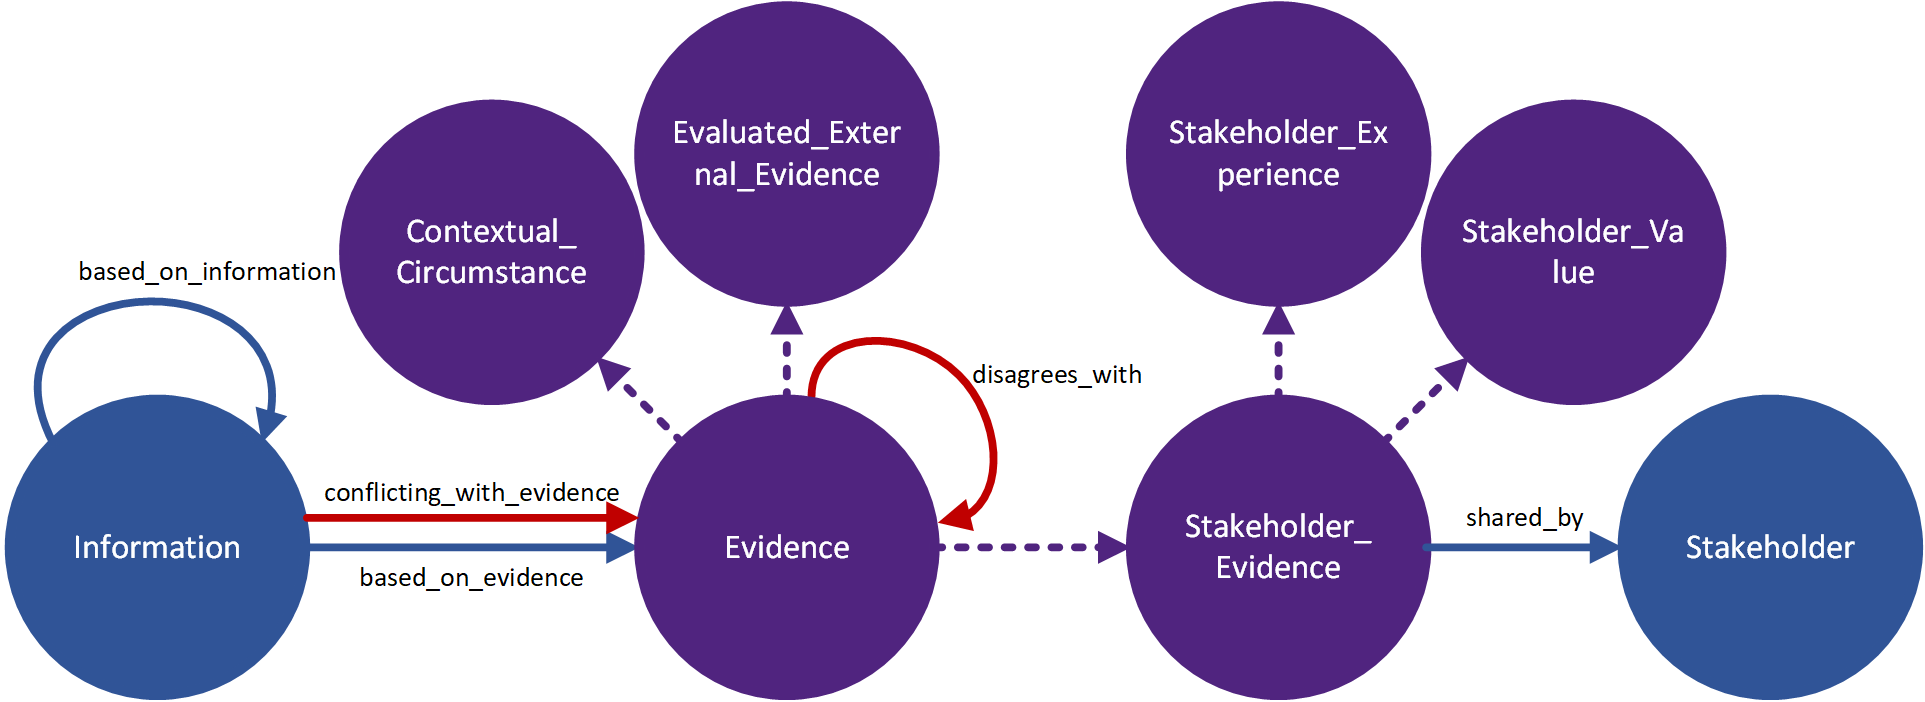
\includegraphics[width=14cm]{../../Images/04_Contribution/04_Conflict_Ontology.png}
  \caption{The conflict pattern uses the reproducibility pattern and extends it with the object property $disagrees\_with$. Code sample \ref{GODP_CONF_LEV} presents the GDOL code for instantiating the conflict pattern.}
  \label{fig:conflict}
\end{figure}

\paragraph{Inferencing}
We introduce an additional object property: $conflict\_with\_evidence$. When we base $In{\f}ormationX$ on $EvidenceA$, and $EvidenceA$ disagrees with $EvidenceB$, $In{\f}ormationX$ conflicts with $EvidenceB$. This conflict reduces trust in $In{\f}ormationX$. Figure \ref{fig:conflict_inferred} presents the super property that infers this knowledge from the existing ontology structure.

\begin{figure}[H]
\centering
  
\includegraphics[width=17cm]{../../Images/Conflict_Inferred.png}
  \caption{The configuration of the super property that infers the object property $conflict\_with\_evidence$ in Prot\'eg\'e.}
  \label{fig:conflict_inferred}
\end{figure}

$disagrees\_with$ is symmetric and irreflexive. Disagreement is always symmetric: if $StakeholderA$ disagrees with $StakeholderB$ on a specific subject, then $StakeholderB$ also disagrees with $StakeholderA$. Figure \ref{fig:conflict_irreflexive} presents the situation in which $disagrees\_with$ is symmetric and irreflexive.

\begin{figure}[H]
\centering
  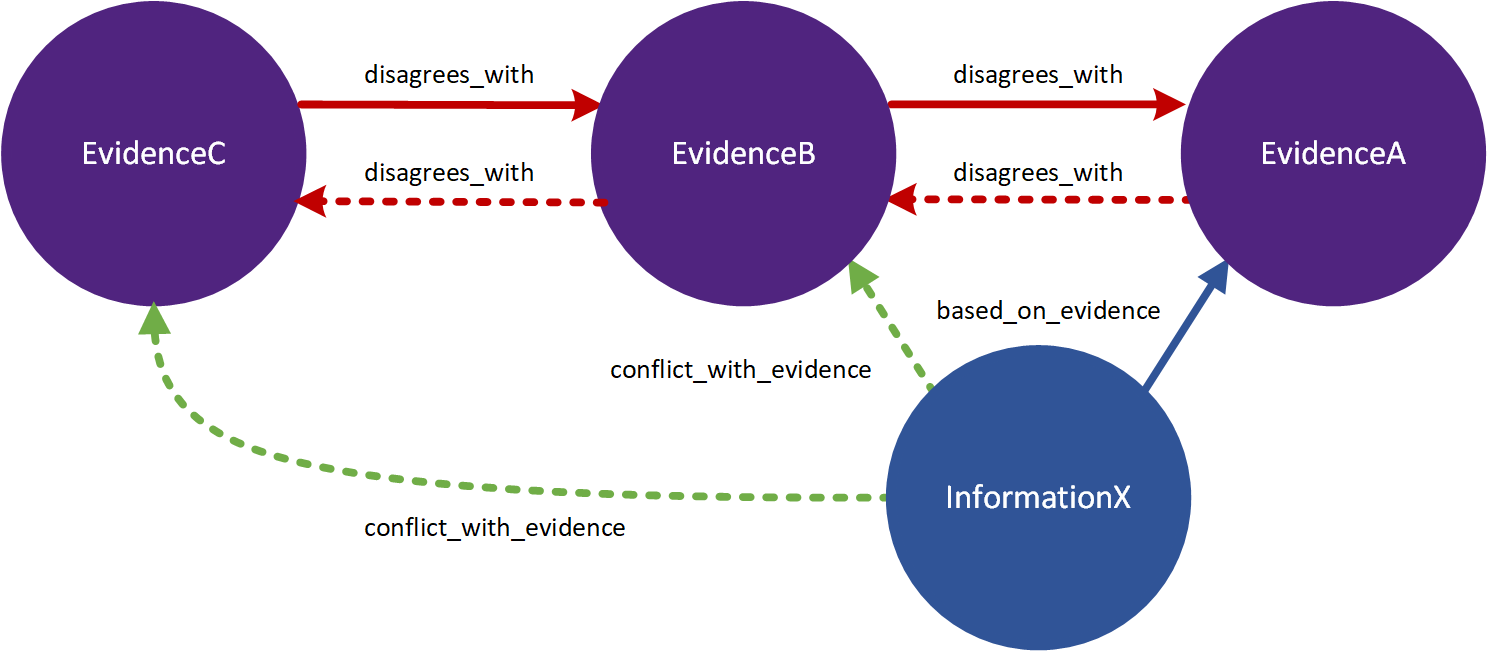
\includegraphics[width=13cm]{../../Images/04_Contribution/04_Conflict_Characteristics.png}
  \caption{The symmetric and irreflexive characteristics of $disagrees\_with$. The reasoner infers the dotted lines based on the super property figure \ref{fig:conflict_inferred} presents.}
  \label{fig:conflict_irreflexive}
\end{figure}

\paragraph{Inconsistency}
The consensus pattern inherits the consistency validation from the reproducibility pattern. We describe the consistency of the reproducibility pattern in section \ref{rep_incons} \nameref{rep_incons}.

Figure \ref{fig:conflict_transitive} presents the hypothetical situation in which $disagrees\_with$ is symmetric, transitive, and irreflexive. This situation results in an inconsistent ontology. The reasoner infers the $disagrees\_with$ object property on $EvidenceA$ based on the transitivity characteristic. This object property causes conflict with the irreflexive character of $disagrees\_with$. The transitivity helps us to discover disagreement chains and ensures we present the right conflict level to the decision-maker. Transitivity causes a problem: evidence cannot disagree with itself. When we combine the irreflexive and transitive characteristics, the reasoner might infer the $disagrees\_with$ object property on an evidence source. For example, we assume $R$ is transitive and irreflexive. By transitivity, we conclude $xRy \land yRx \rightarrow xRx$. However, this is not possible as $R$ should be irreflexive as well.

\begin{figure}[H]
\centering
  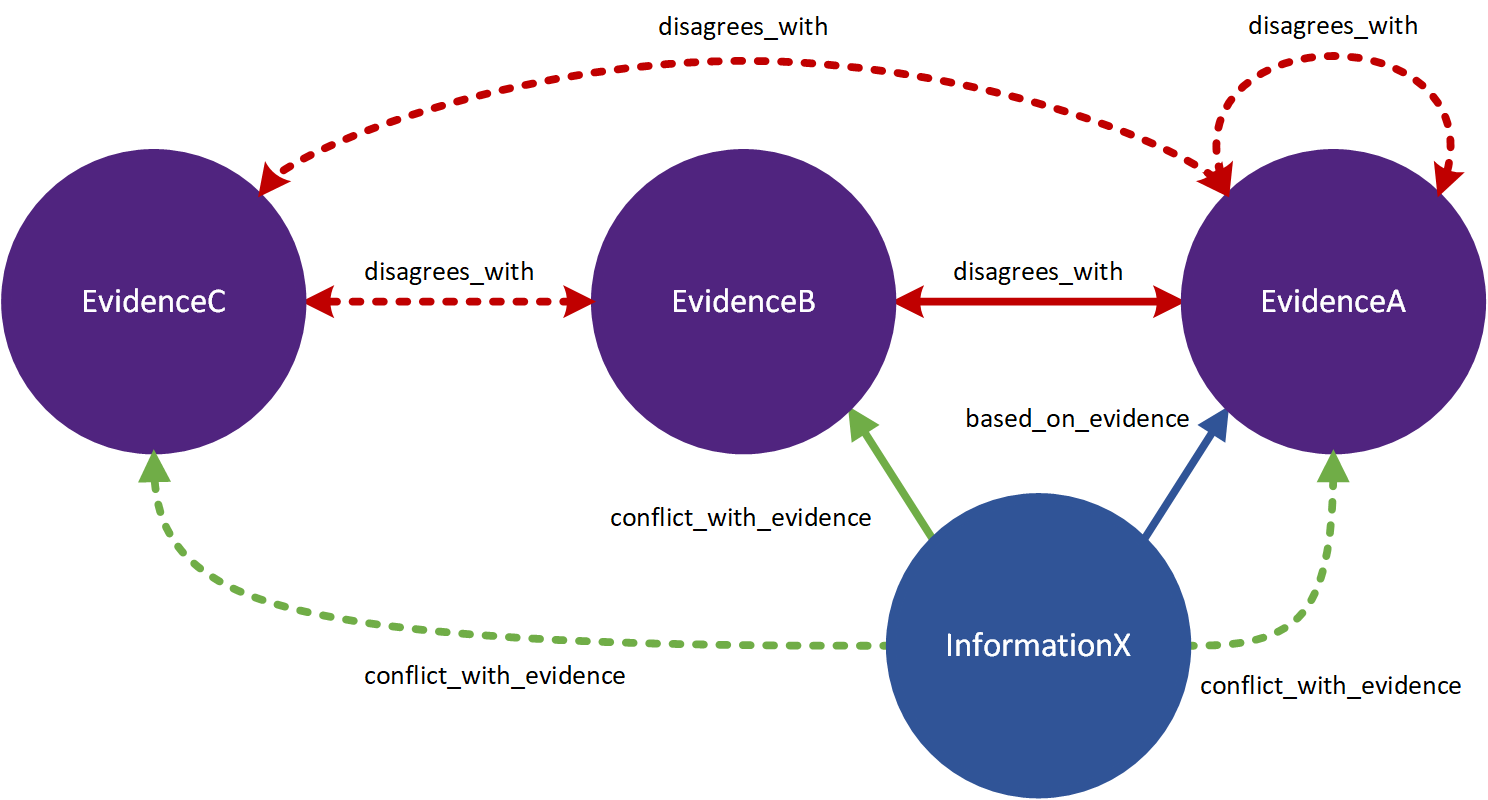
\includegraphics[width=13cm]{../../Images/Conflict_Transitive.png}
  \caption{The transitive characteristic of $disagrees\_with$ causes an inconsistent ontology. The reasoner infers the dotted lines based on the super property figure \ref{fig:conflict_inferred} presents.}
  \label{fig:conflict_transitive}
\end{figure}

\paragraph{Generic ontology design pattern}
Code sample \ref{GODP_CONF_LEV} presents the described solution into GDOL. We take the $Reproducibility\_Basic$ pattern and add the $disagrees\_with$ and $conflict\_with\_evidence$ object properties.

\begin{lstlisting}[float,language=GDOL,caption={The GDOL code that extends the reproducibility pattern and results in the conflict pattern. We take the $Reproducibility\_Basic$ pattern and add the $disagrees\_with$ and $conflict\_with\_evidence$ object properties.},label={GODP_CONF_LEV}][H]
ontology Conflict = Reproducibility_Basic then
  ObjectProperty: disagrees_with Domain: Evidence Range: Evidence Characteristics: Symmetric, Irreflexive
  ObjectProperty: conflict_with_evidence SubPropertyChain: based_on_evidence o disagrees_with SubPropertyOf: conflict_with_evidence
end
\end{lstlisting}

\paragraph{Constraints}
The conflict pattern requires the definition of a conflict level. Conflict reduces the reliability of the information and evidence. Therefore, we do not accept any conflict for our evidence and define the maximum conflict-level as $0$. Any conflict that the constraints detect immediately causes a violation. We use the cardinality constraint $sh:minCount$ for this detection: each individual classified as $In{\f}ormation$ should not have any path (object property) $conflict\_with\_evidence$.

\begin{lstlisting}[float,language=SHACL,caption={The SHACL shapes that detect if there is conflict. },label={SHACL_CONF_LEV}][H]
Used_InformationShape a sh:NodeShape;
	sh:targetClass Used_Information; 
	sh:property [
		sh:path conflict_with_evidence; 
		sh:severity sh:Violation; 
		sh:maxCount 0; 
		sh:message "Conflict detected. Please resolve the conflict or re-consider using this information."; ];
\end{lstlisting} 

\subsubsection{Pattern consolidation}
The decision ontology pattern reduces the complexity of the instantiation of the completeness, reproducibility, consensus, and conflict patterns.

\paragraph{Pattern dependencies}
We cannot reproduce information that does not exist. We validate the reproducibility of existing, and therefore, complete information. The consensus and conflict patterns have a similar dependency on the reproducibility pattern. When information is evidence-based, we can validate if the evidence agrees with other evidence (and define the level of consensus) or if information disagrees with other evidence (and define the level of conflict). 

\begin{center}
\large\color{document}{There is no consensus or conflict without reproducibility. There is no reproducibility without completeness.} 
\end{center}

\paragraph{Completeness and reproducibility using N-ary relations}
The completeness pattern validates the completeness of data properties and object properties. The reproducibility pattern validates the reproducibility of individuals using the object properties $based\_on\_evidence$ and $based\_on\_in{\f}ormation$. We need to relate a data property, containing decision-relevant information, to an object property. Figure \ref{fig:DecisionDesignPattern_NARY1} presents an example: $dataproperty1$ would be reproducible based on $based\_on\_evidence$. However, $dataproperty2$ would not be reproducible.

\begin{figure}[H]
\centering
  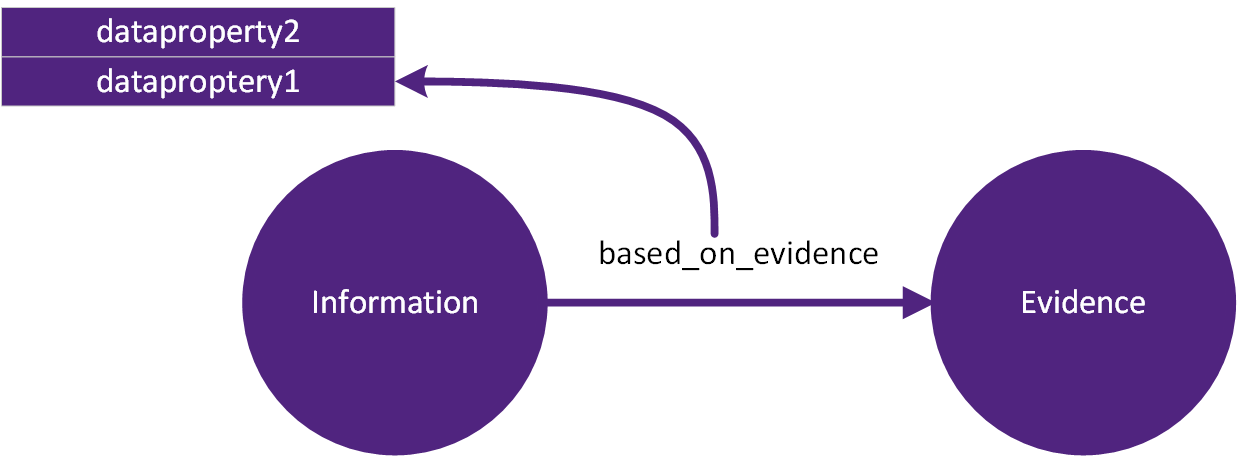
\includegraphics[width=10cm]{../../Images/04_Contribution/04_DecisionDesignPattern_NARY1.png}
  \caption{How can we reproduce $dataproperty1$ based on the object property $based\_on\_evidence$? However, $dataproperty2$ is not reproducible.}
  \label{fig:DecisionDesignPattern_NARY1}
\end{figure}

A property is a binary relation that relates two individuals \parencite{WEB16}. This concept makes it challenging to describe a relationship. In our case, we would describe the $based\_on\_evidence$ relationship with the data properties this relationship represents. We can describe object properties using annotations. Figure \ref{fig:DecisionDesignPattern_NARY2} presents the implementation of the annotation on the object property $based\_on\_evidence$ in Prot\'eg\'e, indicating that it $reproduces$ the $requirement\_cost$. 

\begin{figure}[H]
\centering
  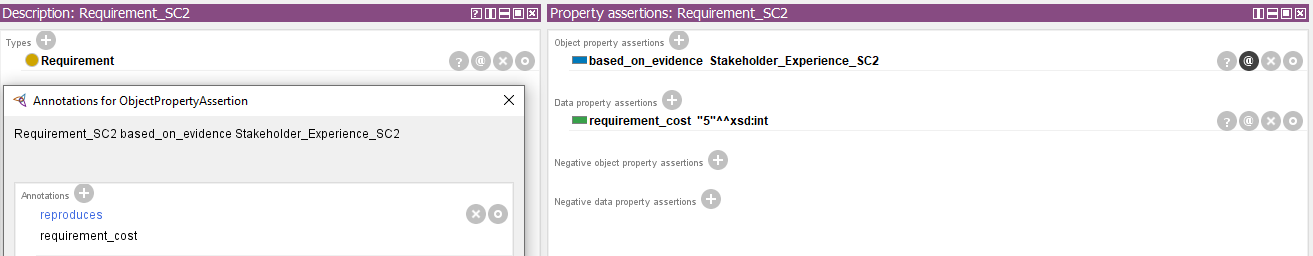
\includegraphics[width=16cm]{../../Images/04_Contribution/04_DecisionDesignPattern_NARY2.png}
  \caption{The implementation of the annotation on the object property $based\_on\_evidence$ in Prot\'eg\'e, indicating that it $reproduces$ the $requirement\_cost$.}
  \label{fig:DecisionDesignPattern_NARY2}
\end{figure}

However, annotation properties are merely descriptive and cannot define a characteristic of an object or data property \parencite{WEB12}. Therefore, the annotation properties are not suitable for inferencing or constraint validation. Additionally, we cannot use annotation properties to validate the reproducibility.

We define n-ary relations to solve this challenge \parencite{WEB16}. An n-ary relation introduces a new class for information that we would typically store in a data property. The new class hosts the actual information as data properties. We define three types of individuals for our purpose: $root$, $in{\f}ormation$, and $target$. The $root$ provides the context for the $in{\f}ormation$. The $in{\f}ormation$ stores the actual information in two data properties ($data\_value$ and $data\_description$), and the $target$ serves as the target for reproduction. We use the $data\_value$ to give an integer to the information. The $data\_description$ describes the value. We suggest setting the $data\_value$ to $0$ when the context does not require the use of the $data\_value$. Figure \ref{fig:root_information_target} presents the definitions.

\begin{figure}[H]
\centering
  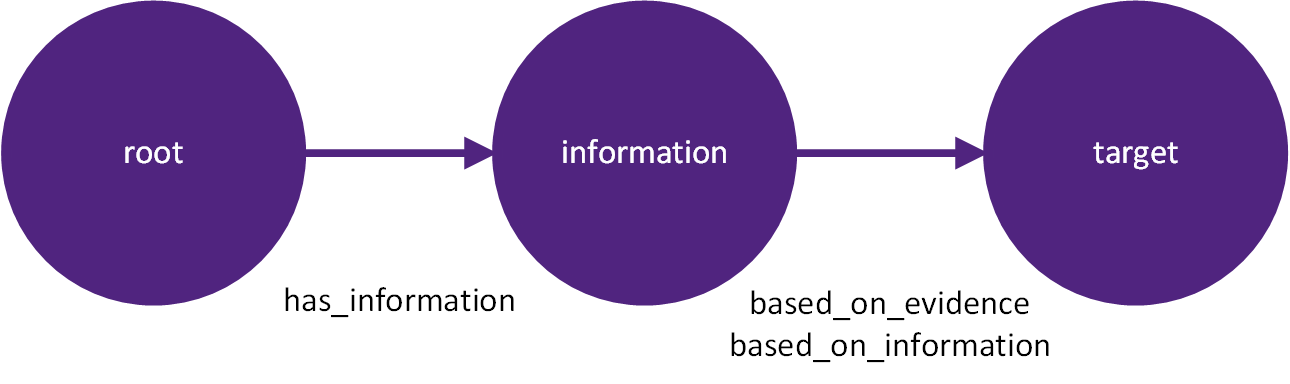
\includegraphics[width=10cm]{../../Images/04_Contribution/04_root_information_target.png}
  \caption{The $root$, $in{\f}ormation$, and $target$ individuals in n-ary relation.}
  \label{fig:root_information_target}
\end{figure}

Figure \ref{fig:DecisionDesignPattern_NARY3} presents an example of this concept. Class $r$, the root class, has two decision-relevant information properties: $n1$ and $n2$. These decision-relevant information properties have at least the $data\_value$ and $data\_description$ data properties. We classify them as $In{\f}ormation$. $n1$ and $n2$ are reproducible using the object properties $based\_on\_evidence$ or $based\_on\_in{\f}ormation$. We need to ensure that the completeness and reproducibility patterns function in this environment.

\begin{figure}[H]
\centering
  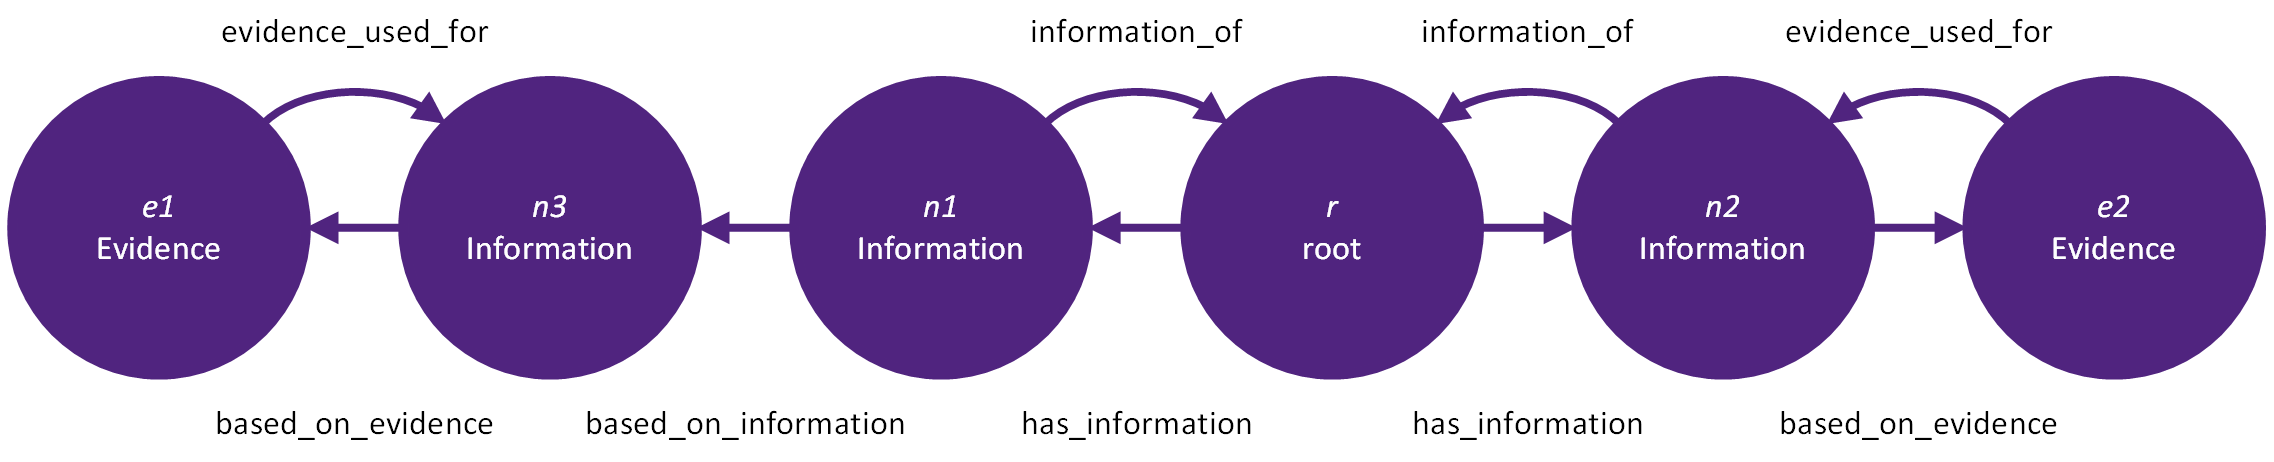
\includegraphics[width=17cm]{../../Images/04_Contribution/04_DecisionDesignPattern_NARY3.png}
  \caption{Class $r$ with two decision-relevant information properties: $n1$ and $n2$. These decision-relevant information properties have a $data\_value$ and a $data\_description$. $n1$ and $n2$ are reproducible using the object property $based\_on\_evidence$.}
  \label{fig:DecisionDesignPattern_NARY3}
\end{figure}

We validate the completeness of information using the $has\_information$ object property, including its range. We validate the reproducibility of information using the $based\_on\_evidence$ and $based\_on\_in{\f}ormation$ object properties.

\paragraph{\emph{Used} classes}
We use $Used\_*$ classes throughout the patterns to define the scope of the constraints. Each $Used\_*$ class is a subclass of its parent. We define the $Used\_*$ class in a way the reasoner classifies individuals that are relevant for the constraints. Figure \ref{fig:04_Used_Information} presents, for example, the $Used\_In{\f}ormation$ class. There might be a lot of individuals classified as $In{\f}ormation$. However, these individuals are only relevant to the decision-maker if the decision-maker uses them. The reasoner classifies individuals as $Used\_In{\f}ormation$ when they have the $in{\f}ormation\_of$ object property. We use the inverse of the $has\_in{\f}ormation\_*$ object property to infer that information is used in the context of a decision-relevant root individual. We use the $evidence\_used\_for$ object property to infer $Used\_Evidence$ similarly.  

\begin{figure}[H]
\centering
  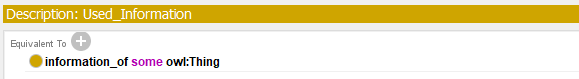
\includegraphics[width=12cm]{../../Images/04_Contribution/04_Used_Information.png}
  \caption{The $Used\_In{\f}ormation$ configuration in Prot\'eg\'e. The reasoner classifies individuals as $Used\_In{\f}ormation$ when they have the $in{\f}ormation\_of$ object property.}
  \label{fig:04_Used_Information}
\end{figure} 

\paragraph{Inferencing}
We use inferencing in the decision design pattern to infer the information types from the object property $has\_information\_*$. The completeness pattern uses the information generated by the reasoner to validate the existence of specific data properties. Figure \ref{fig:04_DDP_Inference} presents an example in which individual $A$ is connected to individual $B$ by $has\_information\_temperature$. We set the range of $has\_information\_temperature$ to the class $Temperature$. As a result, the reasoner infers that $B$ must be of type $Temperature$. This mechanism allows the completeness pattern to validate if individuals classified as $Temperature$ have specific data or object properties.

\begin{figure}[H]
\centering
  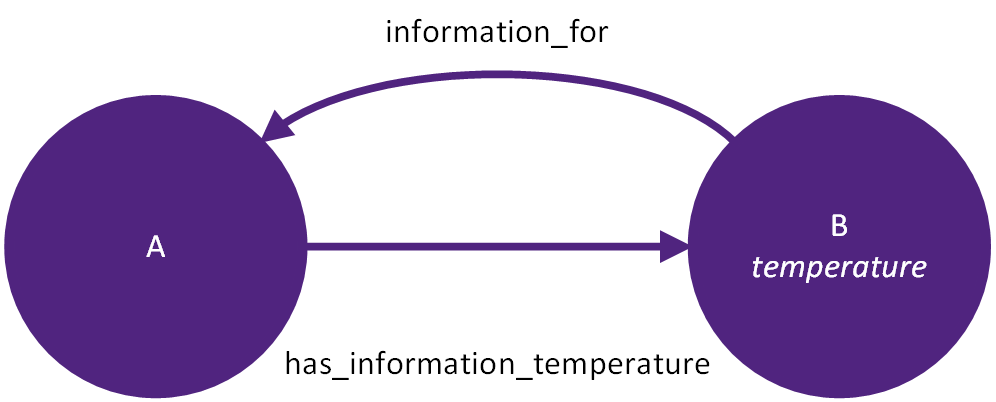
\includegraphics[width=8cm]{../../Images/04_Contribution/04_DDP_Inference.png}
  \caption{An example in which individual $A$ is connected to individual $B$ by $has\_information\_temperature$. We set the range of $has\_in{\f}ormation\_temperature$ to the class $Temperature$. As a result, the reasoner infers that $B$ must be of type $Temperature$.}
  \label{fig:04_DDP_Inference}
\end{figure}

\paragraph{Inconsistency}
We guard the consistency of the ontology using $DisjointClasses$. The $agrees\_with$ and $disagrees\_with$ object properties of the consensus and conflict patterns are naturally disjoint: when evidence $A$ agrees with evidence $B$, they cannot disagree at the same time. The decision design pattern inherits other inconsistency prevention mechanics from the completeness, reproducibility, consensus, and conflict patterns.

\paragraph{Generic ontology design pattern} \label{dop-godp}
The decision ontology pattern instantiates the completeness, reproducibility, consensus, and conflict patterns. These patterns have an overlap in their instantiation; for example, the consensus and conflict pattern both instantiate the $Reproducibility\_Base$. We reduce the overlap by defining new instantiation code. Code sample \ref{GODP_DDP_Instantiation_Basic} presents the instantiation code for the base ontology structure. The base instantiation code addresses the reproducibility, consensus, conflict, and a part of the completeness pattern. The base instantiation does not use any parameters.

\begin{lstlisting}[float,language=GDOL,caption={The base GDOL instantiation code for the decision ontology pattern. The instantiation code is a combination of the completeness, reproducibility, consensus, and conflict patterns.},label={GODP_DDP_Instantiation_Basic}][H]
pattern DecisionOntologyPattern_Basic = Reproducibility_Basic then
 %% Consensus pattern without reproducibility pattern
 ObjectProperty: agrees_with Domain: Evidence Range: Evidence Characteristics: Transitive, Symmetric
 ObjectProperty: based_on_evidence SuperPropertyOf: based_on_evidence o agrees_with SubPropertyOf: based_on_evidence
 %% Conflict pattern without reproducibility pattern
 ObjectProperty: disagrees_with Domain: Evidence Range: Evidence Characteristics: Symmetric, Irreflexive
 ObjectProperty: conflict_with_evidence SuperPropertyOf: based_on_evidence o disagrees_with SubPropertyOf: conflict_with_evidence
 %% Completeness pattern
 Completeness_dp [data_value][Information][xsd:int] %% Data property and information class as parameters
 Completeness_dp [data_description][Information][xsd:string] %% Data property and information class as parameters
 %% Used information
 Object Property: information_of InverseOf: has_information
 Class: Used_Information EquivalentTo: information_of some owl:Thing
 %% Used evidence
 Object Property: evidence_used_for InverseOf: based_on_evidence
 Class: Used_Evidence EquivalentTo: evidence_used_for some Information 
\end{lstlisting}
 
Figure \ref{fig:DecisionDesignPattern} presents the instantiated decision ontology pattern. This ontology does not include context. We took the \textcolor{Violet}{violet} edges and nodes from the evidence-based management pattern, the \textcolor{DarkBlue}{blue} edges and nodes from the reproducibility pattern, the \textcolor{Red}{red} edges from the conflict pattern, and the \textcolor{Green}{green} edge from the consensus pattern. The completeness pattern does not include structural elements.
 
\begin{figure}[H]
\centering
  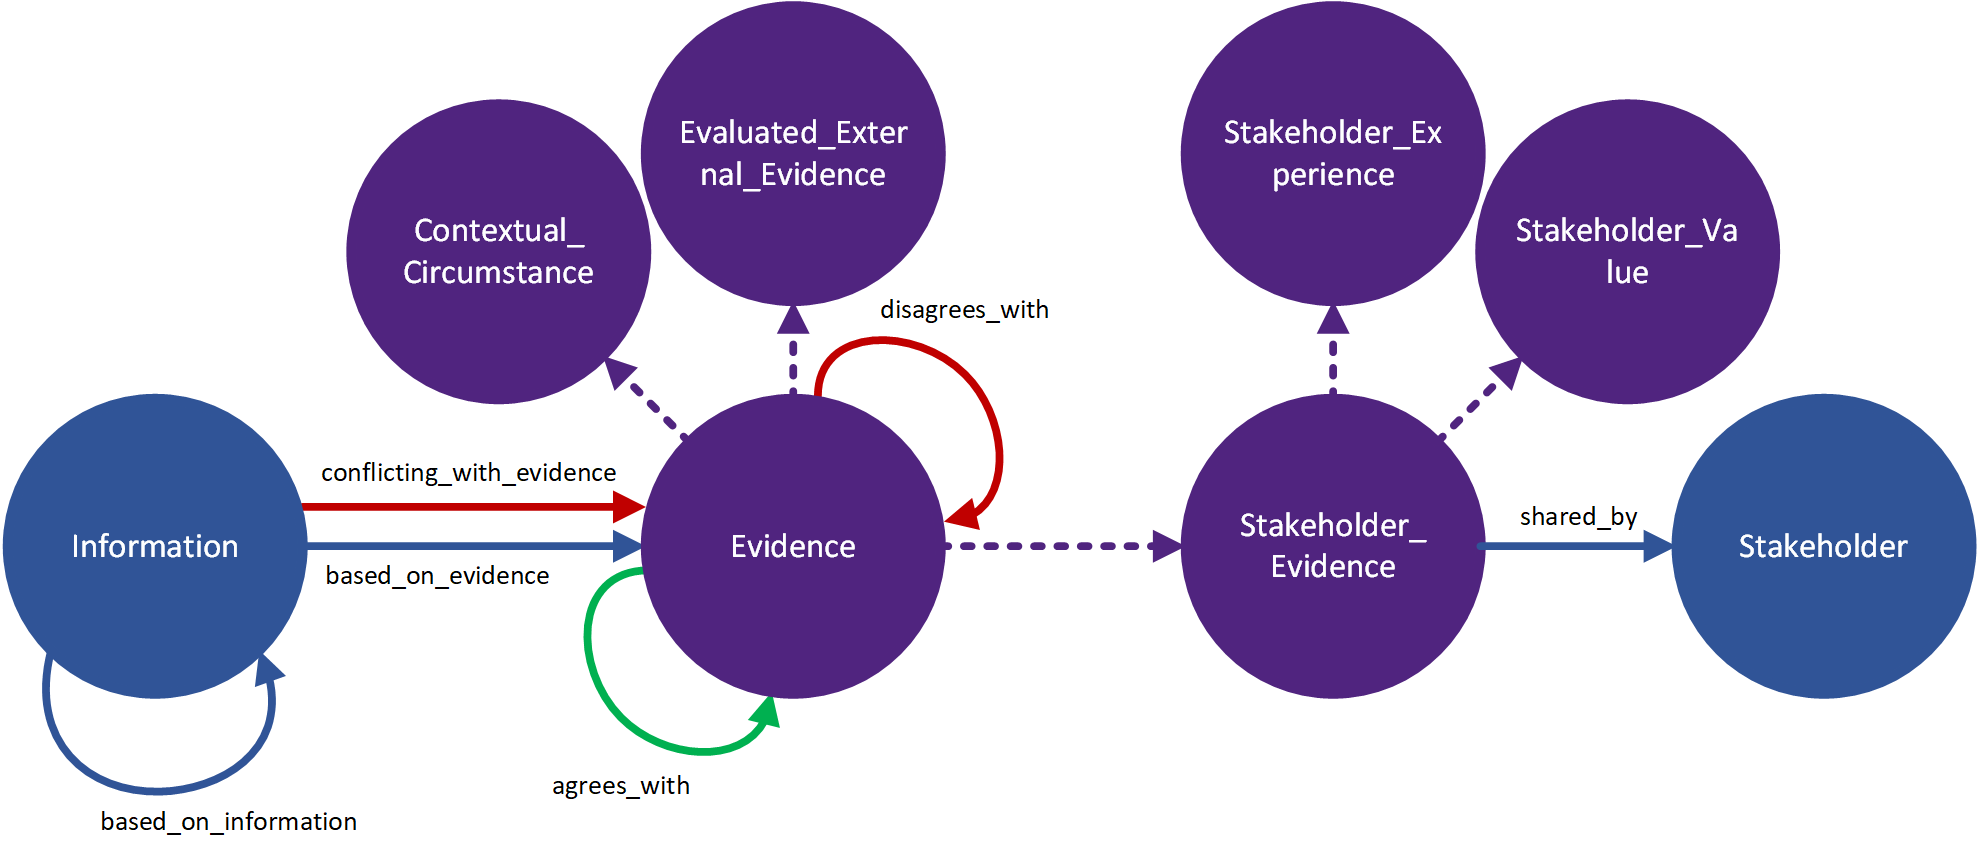
\includegraphics[width=15cm]{../../Images/04_Contribution/04_DecisionDesignPattern.png}
  \caption{The instantiated decision ontology pattern without context. We took the \textcolor{Violet}{violet} edges and nodes from the evidence-based management pattern, the \textcolor{DarkBlue}{blue} edges and nodes from the reproducibility pattern, the \textcolor{Red}{red} edges from the conflict pattern, and the \textcolor{Green}{green} edge from the consensus pattern.}
  \label{fig:DecisionDesignPattern}
\end{figure}

The completeness and reproducibility patterns require a context-specific instantiation. We instantiate a new context-specific ontology structure for every information type that decision-makers use to make a decision. We use parameter $i$ to represent this class. Code sample \ref{GODP_DDP_Instantiation_Context} presents the context-specific instantiation code. 

\begin{lstlisting}[float,language=GDOL,caption={The context-specific GDOL instantiation code to instantiate the decision design pattern. The code is a combination of the context-specific instantiation code of the completeness and reproducibility patterns.},label={GODP_DDP_Instantiation_Context}][H]
pattern DecisionOntologyPattern_Context [Class: i; Class: r] = 
 Completeness_op[has_information[i]; r; i] %% Object property, root class, and information class as parameters
\end{lstlisting}

\paragraph{Constraints}
We need to combine the basic and context-dependent constraints of the completeness, reproducibility, consensus, and conflict patterns. The constraints of the reproducibility and conflict patterns target the $Used\_In{\f}ormation$ class. Code sample \ref{SHACL_DDP_Basic} combines the constraints for these two patterns into one SHACL shape. 

\begin{lstlisting}[float,language=SHACL,caption={This code sample combines the constraints of the reproducibility, consensus, and conflict patterns. We have merged parts of the reproducibility and consensus patterns.},label={SHACL_DDP_Basic}][H]
UsedInformationShape a sh:NodeShape;
	sh:targetClass Used_Information; 
	sh:property [
		sh:or (
			[sh:path based_on_information; sh:minCount 1;]
			[sh:path based_on_evidence; sh:minCount 1;]
		)
		sh:severity sh:Violation; 
		sh:minCount 1; 
		sh:message "Reproducibility: increase the number of evidence sources for this information."; ];
	sh:targetClass Information; 
	# Conflict pattern
	sh:property [
		sh:path conflict_with_evidence; 
		sh:severity sh:Violation; 
		sh:maxCount 0; 
		sh:message "Conflict detected. Please resolve the conflict or re-consider using this information."; ];
\end{lstlisting}

Code sample \ref{SHACL_REP_SH} is part of the reproducibility pattern and presents the constraints that validate if $Stakeholder\_Evidence$ is $shared\_by$ a stakeholder. Code sample \ref{SHACL_CON_LEV} presents the constraints that validate the consensus pattern. We include both code samples as-is into the decision ontology pattern.

We instantiate the contextual constraints multiple times per scenario, depending on the need of the scenario. The completeness pattern is context-sensitive. Code sample \ref{SHACL_COM_DP} presents the only context-sensitive constraints we use in the decision design pattern.
\subsection{Decision presentation pattern} \label{odp_decision_presentation}
The outcome of a decision might deviate from the expectations of the decision-maker when the information maturity-level is low. This deviation is not a big problem when the impact of the decision on the organisation is low. However, when the impact of the decision on the organisation is high, the decision-maker wants more certainty that the decision reaches the expected outcome. There is a consensus on the benefits of evidence-based decision-making. However, \cite{DM03} and \cite{DM07} also raise the need for more research to prove its effectiveness.

\begin{center}
\large\color{document}{The decision presentation pattern helps decision-makers to make evidence-based decisions by presenting the information maturity-level.} 
\end{center}

The decision presentation pattern achieves this goal by enabling the decision-maker to understand the maturity-level of the decision-relevant information. We give decision-makers two options when we present the information maturity-level:
\begin{enumerate}
\item Accept the status of the decision-relevant information.
\item Elaborate further on the decision-relevant information.
\end{enumerate}

We enable the decision-maker to understand which information requires more elaboration. This elaboration can increase the completeness and reliability of the information. We present three dashboards for the decision-maker. The first dashboard presents the information maturity-level and evidence spread for all the decision-relevant information. The second dashboard presents the information maturity-level for the completeness, reproducibility, consensus, and conflict patterns. The third dashboard presents the maturity-levels per individual. 

Figure \ref{fig:04_Presentation_Components} presents a navigation concept for the three dashboards. The decision-maker can browse from the first dashboard to the second dashboard, from the second dashboard to the third dashboard, and from the first dashboard to the third dashboard. The context of the third dashboard changes depending on the origin of the decision-maker. For example, if the decision-maker browses from dashboard two to dashboard three using the completeness maturity-level, dashboard three presents the completeness of the decision-relevant information per individual.

\begin{figure}[H]
\centering
  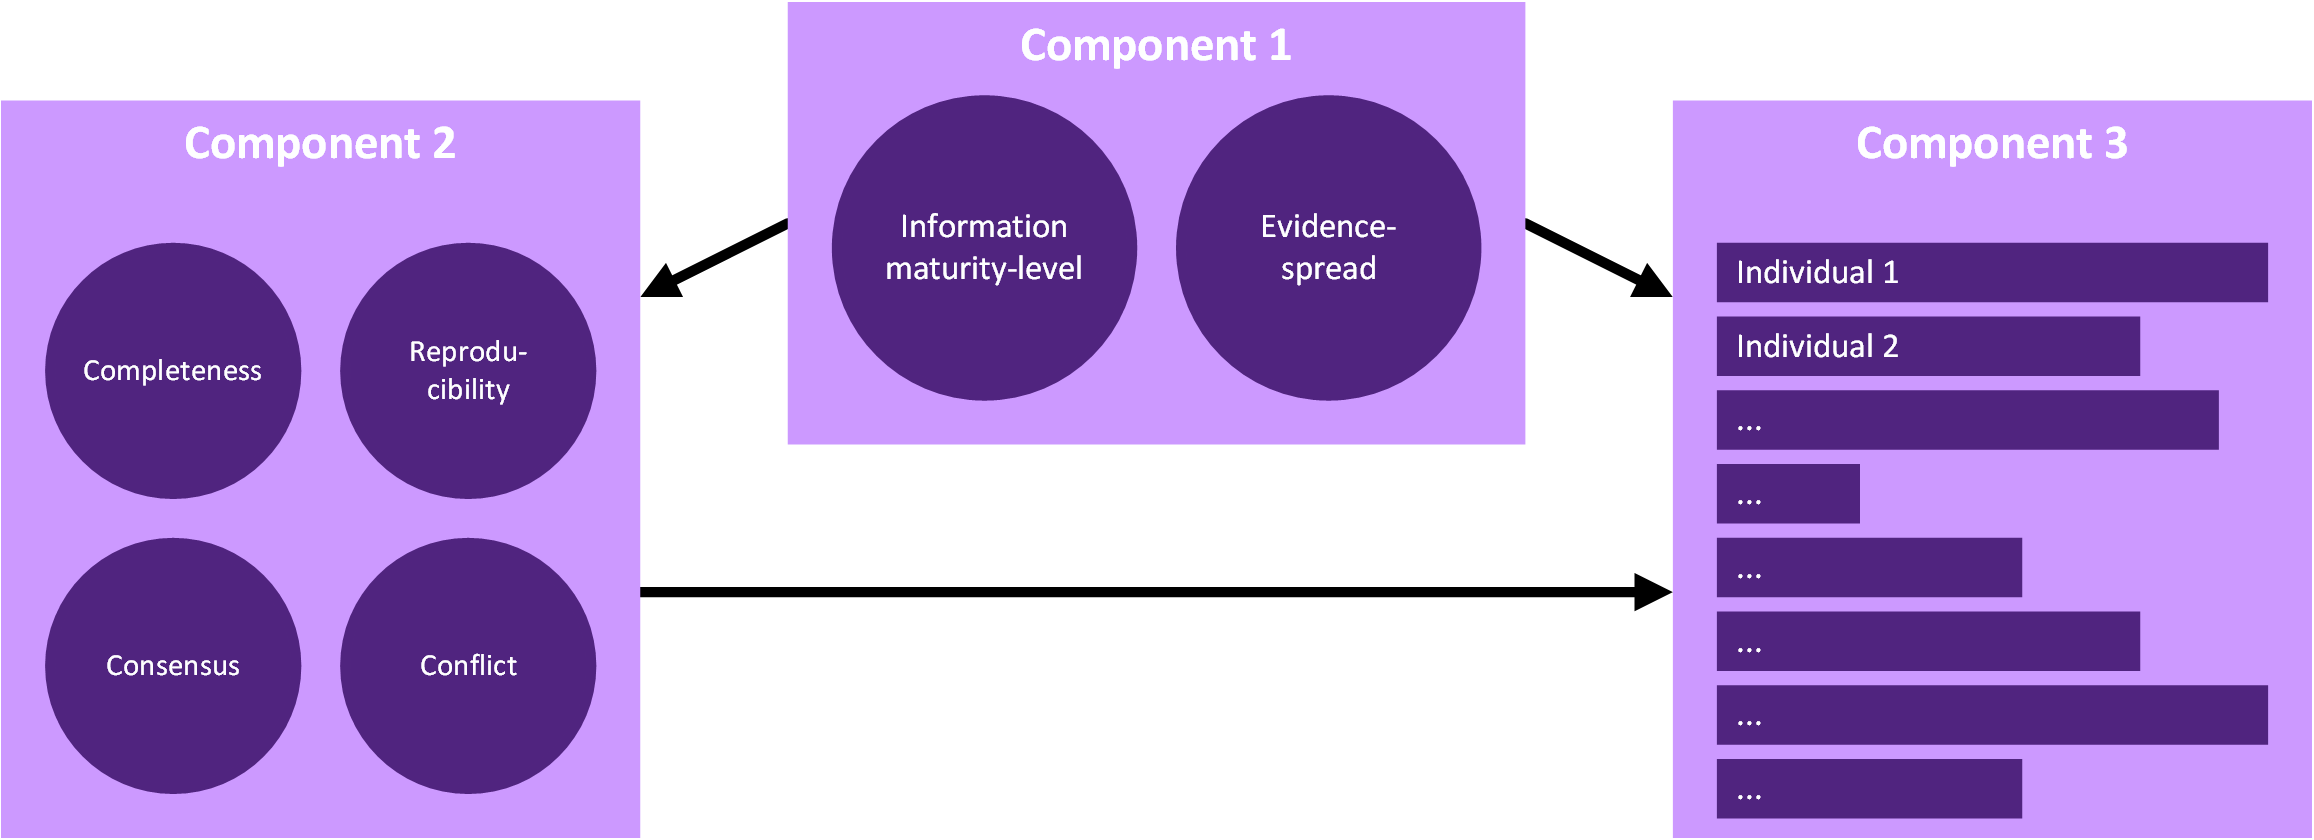
\includegraphics[width=16cm]{../../Images/04_Contribution/04_Presentation_Components.png}
  \caption{The three presentation dashboards that allow a decision-maker to understand the information-maturity level and evidence-spread.}
  \label{fig:04_Presentation_Components}
\end{figure} 

\subsubsection{Dashboard 1: Consolidated information maturity-level and evidence spread} \label{odp_maturity_evidence_spread}
The goal of the first dashboard is to help decision-makers to decide if the information maturity-level and evidence-spread are acceptable in the context of the specific decision. We determine an average information maturity-level and evidence-spread across the decision-relevant root individuals. Figure \ref{fig:root_information_target_1} repeats the definition of the root, information, and target individuals.

\begin{figure}[H]
\centering
  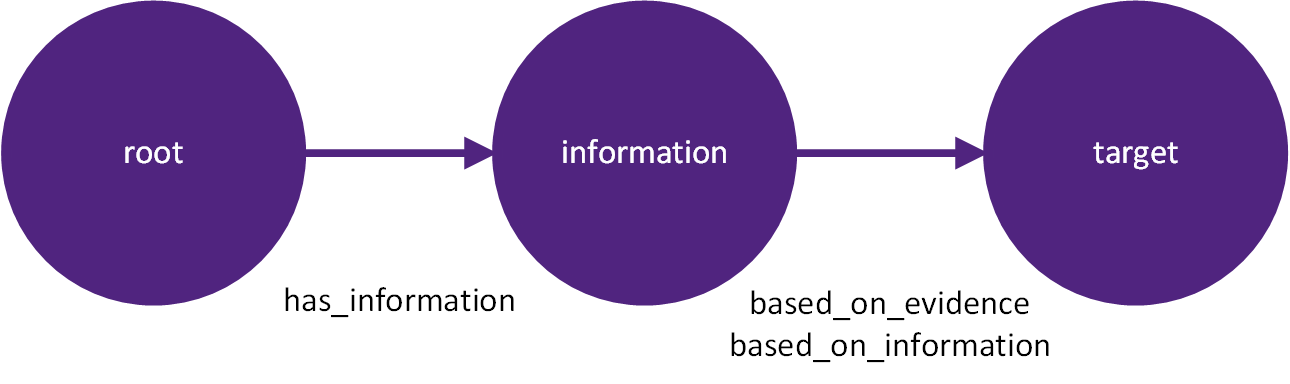
\includegraphics[width=10cm]{../../Images/04_Contribution/04_root_information_target.png}
  \caption{The $root$, $in{\f}ormation$, and $target$ individuals in n-ary relation.}
  \label{fig:root_information_target_1}
\end{figure}

We need to know the maximum number of violations before we can determine the information maturity-level. The maximum number of violations depends on the decision-relevant root individuals. We create a set $RI$ that contains the decision-relevant root individuals. The contents of the set $RI$ depend on the context of the decision. Therefore, we cannot define $RI$ as part of the pattern.  

\paragraph{Maximum number of violations: Completeness}
The maximum number of violations for the completeness pattern for a specific decision-relevant root individual depends on three things: 
\begin{enumerate}
\item The required $has\_in{\f}ormation\_*$ object properties.
\item The availability of the $data\_value$ and $data\_description$ data properties.
\item The availability of context-specific data properties.  
\end{enumerate}

First, we need to retrieve the $has\_in{\f}ormation\_*$ object properties for a specific decision-relevant root individual independent from the ontology content. We need to extract this information manually from the ontology structure by analysing the $has\_in{\f}ormation\_*$ object properties. We represent this manual extraction process in the function $hi(ri) \Rightarrow \mathbb{N}$. $ri$ represents a decision-relevant root individual.

Second, each $has\_in{\f}ormation\_*$ object property leads us to an individual classified as $Information$. Information individuals require a $data\_value$ and $data\_description$. Therefore, we multiply the output of $hi$ by $2$ and add it to the result. 

Third, adding additional object or data properties to the maximum number of violations for the completeness pattern might be necessary. We use variable $c$ for adding the context-specific violations for each decision-relevant root individual.

Equation \ref{eq:mvi1} returns the maximum number of violations for the completeness pattern considering the decision-relevant root individual $ri$ as a parameter: $mvi_1(ri) \rightarrow \mathbb{N}$.

\begin{equation} \label{eq:mvi1}
mvi_1(ri) = hi(ri) + 2hi(ri) + c
\end{equation}

Equation \ref{eq:mv_1} presents the maximum number of violations for the completeness pattern $mv_1$, considering the set of decision-relevant root individuals $RI$. The decision-relevant root individuals are context-dependent. We define a SPARQL query to extract the decision-relevant root individual per scenario.  

\begin{equation} \label{eq:mv_1}
mv_1(RI) = \sum_{ri \in RI} mvi_1(ri)
\end{equation}

\paragraph{Maximum number of violations: Reproducibility}
The maximum number of violations for the reproducibility pattern depends on the number of information classes that require reproduction. We use the same concept to retrieve the maximum number of violations for the reproducibility as we did for the completeness pattern. 

Equation \ref{eq:mvi2} returns the maximum number of violations for the reproducibility pattern considering the decision-relevant root individual $ri$ as a parameter: $mvi_2(ri) \rightarrow \mathbb{N}$.

\begin{equation} \label{eq:mvi2}
mvi_2(ri) = hi(ri)
\end{equation}

Equation \ref{eq:mv_2} presents the maximum number of violations $mv_2$ for the reproducibility pattern considering the set of decision-relevant root individuals $RI$. 

\begin{equation} \label{eq:mv_2}
mv_2(RI) = \sum_{ri \in RI} mvi_2(ri)
\end{equation}

\paragraph{Maximum number of violations: Consensus}
The maximum number of violations for the consensus pattern depends on the maximum number of used evidence sources in the context of a decision. Each evidence source can generate  one violation. Code sample \ref{SPARQL_CONS_IML_ri} presents a SPARQL query that counts the $Used\_Evidence$ individuals based on the object property $evidence\_used\_for$. $evidence\_used\_for$ is the inverse of $based\_on\_evidence$. 

\begin{lstlisting}[float,language=SPARQL1,caption={The SPARQL query that retrieves the number of individuals that the reasoner classified as $Used\_Evidence$ in the context of a specific root class.},label={SPARQL_CONS_IML_ri}][H]
SELECT (COUNT(DISTINCT ?t) as ?count) 
WHERE 
{
	?r has_information ?i .
	?i based_on_evidence ?t .
	?t rdf:type Used_Evidence .
	FILTER (?r = <ri_1>)
}
\end{lstlisting}

Equation \ref{eq:mvi2} returns the maximum number of violations for the reproducibility pattern considering the decision-relevant root individual $ri$ as a parameter: $mvi_3(ri) \rightarrow \mathbb{N}$. Function $uei(ri) \rightarrow \mathbb{N}$ represents the output of the SPARQL query code sample \ref{SPARQL_CONS_IML_ri} presents.

\begin{equation} \label{eq:mvi3}
mvi_3(ri) = uei(ri)
\end{equation}

We cannot sum the results of the individual violations as there might be duplicates in the results. For example, two information individuals might use the same evidence. When counting the maximum number of violations per individual, the sum would count this evidence as two violations. However, considering one decision, one evidence source can generate up to one violation. Code sample \ref{SPARQL_CONS_IML_RI} presents a new filter that we apply on code sample \ref{SPARQL_CONS_IML_ri}. We add the entire content of the set $RI$ to the filter. This way, we ensure that we get a list of evidence sources that is distinct for the specific decision.

\begin{lstlisting}[float,language=SPARQL1,caption={A new filter that we apply on code sample \ref{SPARQL_CONS_IML_ri}. We add the entire content of the set $RI$ to the filter.},label={SPARQL_CONS_IML_RI}][H]
FILTER (?r = <ri_1> || ?r = <ri_2> || ?r = <ri_x>)
\end{lstlisting}

Equation \ref{eq:mv_3} presents the maximum number of violations $mv_3$ for the reproducibility pattern considering the set of decision-relevant root individuals $RI$. Function $ue(RI) \rightarrow \mathbb{N}$ represents the SPARQL query code sample \ref{SPARQL_CONS_IML_RI} presents.

\begin{equation} \label{eq:mv_3}
mv_3(RI) = ue(RI)
\end{equation}

\paragraph{Maximum number of violations: Conflict}
The conflict pattern detects information individuals that have conflicting evidence using the $conflict\_with\_evidence$ object property. The pattern does not care about the number of conflicting evidence related to an individual. Alternatively, we could have used a similar mechanism as we used for the consensus pattern and detect conflict based on the $disagrees\_with$ object property. However, we solve the violation in the consensus pattern by adding an $agrees\_with$ object property to the evidence. The decision-maker can solve the conflict detected by the pattern by removing conflicting evidence or changing the information. In other words, the consensus pattern uses the $Evidence$ class as the core of the solution, while the conflict pattern uses the $Information$ class as the core of the solution.

The maximum number of conflict violations for a decision-relevant root individual depends on the maximum number of information classes that can be evidence-based. We re-use equation $mvi_2$ to determine the maximum number of conflict violations. Equation \ref{eq:mvi24} presents the maximum number of violations $mvi_4$ for the conflict pattern. 

\begin{equation} \label{eq:mvi24}
mvi_2(ri) = mvi_4(ri) = hi(ri)
\end{equation}

Equation \ref{eq:mv_4} presents the maximum number of violations $mv_4$ for the reproducibility pattern considering the set of decision-relevant root individuals $RI$. $mv_4$ is equal to $mv_2$.

\begin{equation} \label{eq:mv_4}
mv_4(RI) = \sum_{ri \in RI} mvi_4(ri)
\end{equation}

\paragraph{Consolidated information maturity-level}
We calculate the information maturity-level using the number of violations detected on the decision-relevant information and the maximum violations. For example, if an individual requires ten object properties and two data properties to be complete, and it triggers two violations, we define the information maturity-level as $(12-2)/12 = 83\%$. Equation \ref{eq:information_maturity_level} includes function $mv(RI) \Rightarrow \mathbb{N}$. This function calculates the maximum number of violations for the set of decision-relevant information. $av(RI) \Rightarrow \mathbb{N}$ calculates the actual number of violations for the set of decision-relevant information and $iml(RI) \Rightarrow \mathbb{N}$ represents the information maturity-level for the set.

\begin{equation} \label{eq:information_maturity_level}
iml(RI) = \dfrac{mv(RI)-av(RI)}{mv(RI)}
\end{equation}

We can easily retrieve the actual number of violations from, for example, Prot\'eg\'e and the SHACL4P plugin. Figure \ref{fig:04_Presentation_IML_SHACL4P} presents an example for which the defined constraints detected two violations for $Opportunity\_SC2\_Vision\_Contribution$. 

\begin{figure}[H]
\centering
  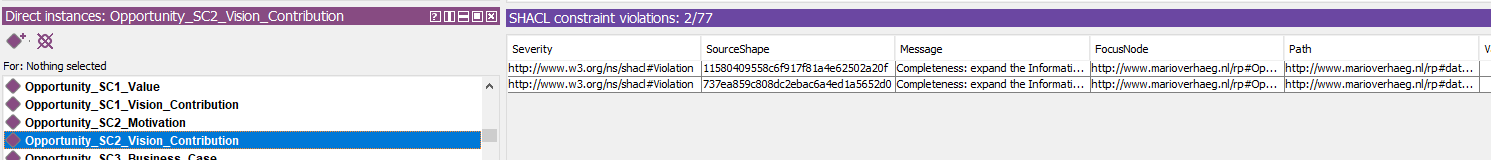
\includegraphics[width=17cm]{../../Images/04_Contribution/04_Presentation_IML_SHACL4P.png}
  \caption{The constraints detect two violations for $Opportunity\_SC2\_Vision\_Contribution$ in Prot\'eg\'e.}
  \label{fig:04_Presentation_IML_SHACL4P}
\end{figure}

Additionally, we need to define the maximum number of violations per decision-relevant root individual and pattern. The maximum number of violations per pattern for a specific individual defines the total maximum number of violations: $mv(RI) = mv_1(RI) + mv_2(RI) + mv_3(RI) + mv_4(RI)$, in which:
\begin{enumerate}
\item $mv_1(RI)$ is the maximum number of violations for the completeness pattern.
\item $mv_2(RI)$ is the maximum number of violations for the reproducibility pattern.
\item $mv_3(RI)$ is the maximum number of violations for the consensus pattern.
\item $mv_4(RI)$ is the maximum number of violations for the conflict pattern
\end{enumerate}

$RI$ represents the set of decision-relevant root individuals.

\paragraph{Evidence spread}
We increase the transparency of the information maturity-level by presenting the evidence spread. For example, a decision entirely based on the evidence type $Stakeholder\_Experience$ might require more elaboration. We use a query to extract the evidence spread from the decision ontology pattern. Within this query, we search for root individuals $ri$ that represent decision-relevant information. The filter in the query accepts multiple root individuals using $||$ the (OR) filter criteria. Code sample \ref{SPARQL_ES} presents the SPARQL query. 

\begin{lstlisting}[float,language=SPARQL1,caption={The SPARQL query that retrieves the evidence spread for decision-relevant information. The SPARQL query counts the individuals that are based on a specific evidence class using type $?t$ of evidence class $?e$.},label={SPARQL_ES}][H]
SELECT ?t (COUNT(DISTINCT ?t) as ?count) 
WHERE 
{
	{
			?ri has_information ?i .
    		?i based_on_evidence ?e .
    		?e rdf:type ?t .
	}
	FILTER(?ri = <ri1> || ?ri = <ri2> || ?rix = <rix> ).
	FILTER(?t != owl:Thing && ?t != Evidence && ?t != Used_Evidence && ?t != Stakeholder_Evidence)
}
GROUP BY ?t
\end{lstlisting}

\paragraph{Overview dashboard}
The goal of the first high-level dashboard is to help the decision-maker answering the question:

\begin{center}
\large\color{document}{Is the information ready for an evidence-based decision?}
\end{center}

This dashboard consists of two charts: the overall information maturity-level and the evidence spread. The information maturity-level helps the decision-maker to understand the quality-level of the information related to this decision. The evidence-spread helps the decision-maker to understand the source of the evidence. The decision-maker needs to find a balance between the information maturity-level and the decision impact, and the evidence-spread and the decision impact. When the impact of a decision is relatively low, the decision-maker might accept a lower information maturity-level and a consolidated evidence-spread. However, when the impact of a decision is relatively high, we expect that decision-makers will require a higher information maturity-level and would like to see a dispersed evidence-spread.

We use a pie-chart to help the decision-maker to understand the mix of evidence-types. The pie-chart is suitable to present relative proportions and percentages \parencite{OTH09}.

We express the information maturity-level as a percentage. Therefore, we use a pie-chart for presenting the information maturity-level as well. Figure \ref{fig:Dashboard_Component_1} presents an example of a dashboard that contains the pie chart presenting the evidence-spread and the information maturity-level. We shorten the time it takes for a decision-maker to consume the information on the dashboard by limiting the number of charts, using data labels to show the actual values, and using a clear legend \parencite{BI09}. Additionally, we use an analogous colour scheme for the evidence spread to ensure the chart appears as one, but the colours are still easily recognisable \parencite{BI10}. The pie chart presenting the information maturity-level uses a different colour scheme, representing \emph{good} (the mature information) and \emph{bad} (the premature information) as \textcolor{LightGreen}{green} and \textcolor{Red}{red}.

\begin{figure}[H]
\centering
  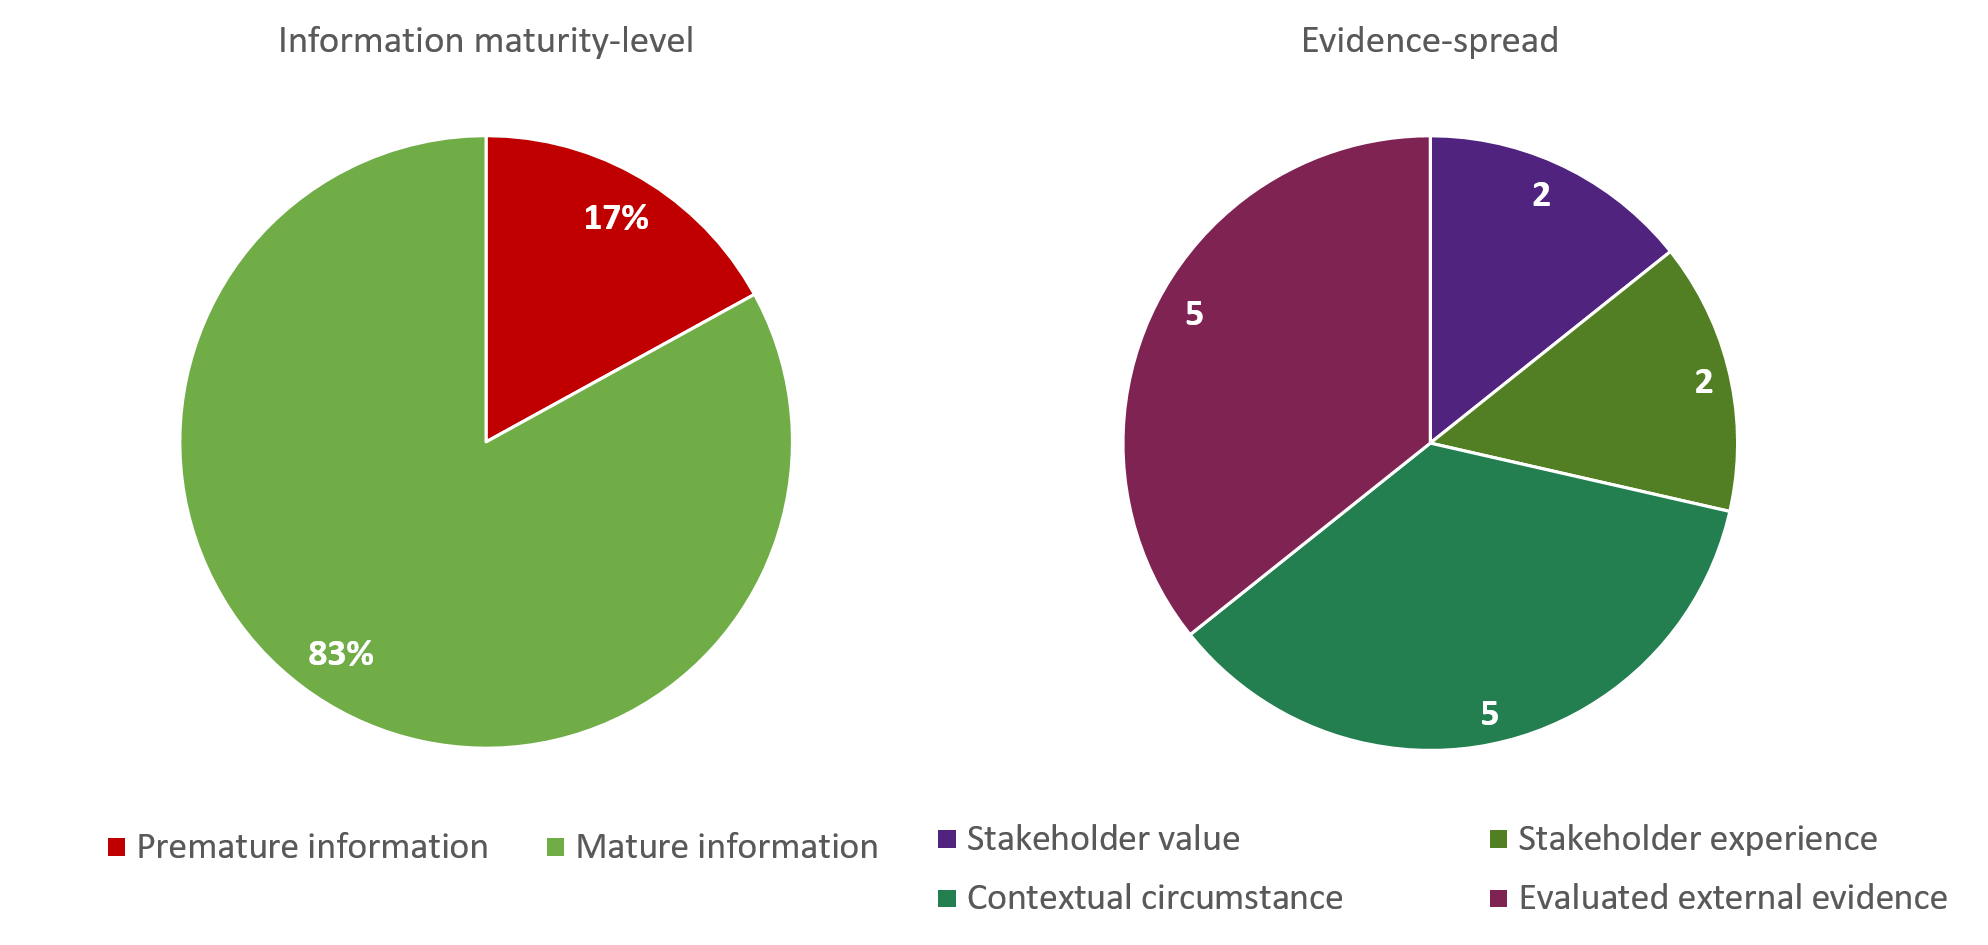
\includegraphics[width=14cm]{../../Images/04_Contribution/Dashboard_Component_1.png}
  \caption{A mock-up of the presentation of the evidence-mix of a specific decision.}
  \label{fig:Dashboard_Component_1}
\end{figure} 

The decision-maker can navigate to the second dashboard by clicking on the pie chart that presents the information maturity-level. Alternatively, the decision-maker can navigate to the third dashboard by clicking on the pie chart that presents the evidence-spread.

\subsubsection{Dashboard 2: Information maturity-level in detail}
The goal of the second dashboard is to enable a decision-maker to understand the consolidated information maturity-level. If the consolidated information maturity-level is lower than expected, the decision-maker can use the second dashboard to understand the root cause. This understanding allows the decision-maker to define actions to improve the information maturity-level. For example, the decision-maker needs to spend time on expanding the information if the completeness pattern causes a low information maturity-level. However, the decision-maker should understand the conflicts and reconsider using conflicting evidence sources if these evidence sources cause a low information maturity-level.

\paragraph{Pattern information maturity-levels}
The detailed information maturity-level consist out of the maturity-level for the completeness, reproducibility, consensus, and conflict patterns. We have defined the functions $mv_1$, $mv_2$, $mv_3$, and $mv_4$ for this. 

In addition to the actual violations $av$, we define $av_1(RI) \Rightarrow \mathbb{N}$, $av_2(RI) \Rightarrow \mathbb{N}$, $av_3(RI) \Rightarrow \mathbb{N}$, and $av_4(RI) \Rightarrow \mathbb{N}$ to represent the actual violations for the completeness, reproducibility, consensus, and conflict patterns. We also define the $avi_x(ri)$ functions that represent the actual violations that a decision-relevant individual generates. Equation \ref{eq:information_maturity_level_x} presents the information maturity-level of the decision-relevant root individuals $RI$ for one of the patterns.

\begin{equation} \label{eq:information_maturity_level_x}
iml_x(RI) = \dfrac{mv_x(RI)-av_x(RI)}{mv_x(RI)}
\end{equation}

\paragraph{Detailed information maturity-level dashboard}
Equation \ref{eq:information_maturity_level_x} defines four pattern-specific information maturity-levels. The pie-chart is most suitable to present percentages and relative proportions \parencite{OTH09}. Figure \ref{fig:Dashboard_Component_2} presents an example of a dashboard that contains the pie charts that present the pattern-specific information maturity-levels. We have made the pie charts easy to understand by tailoring the scales to the specific pattern, representing \emph{good} (the mature information) and \emph{bad} (the premature information) as \textcolor{LightGreen}{green} and \textcolor{Red}{red}, and using data labels. The decision-maker can navigate to the third dashboard by clicking on one of the pie charts. 

\begin{figure}[H]
\centering
  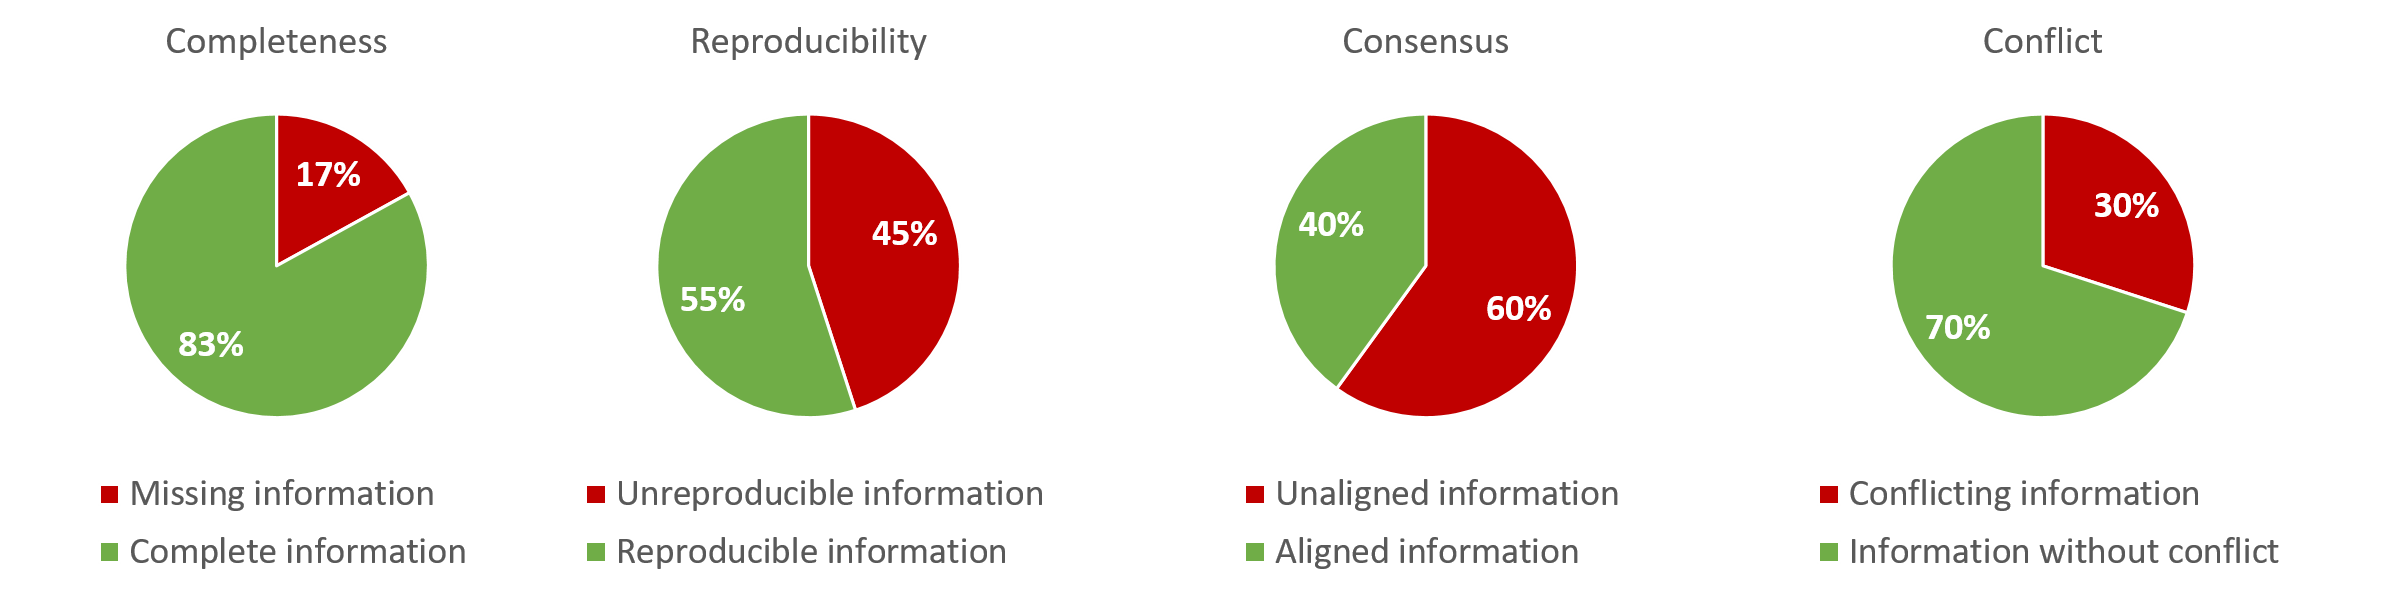
\includegraphics[width=17cm]{../../Images/04_Contribution/Dashboard_Component_2.png}
  \caption{A mock-up of the presentation of the pattern-specific information maturity-levels.}
  \label{fig:Dashboard_Component_2}
\end{figure} 

\subsubsection{Dashboard 3: Violations}
The goal of the third dashboard is to enable the decision-maker to understand which individuals cause the lowered information maturity-level and the evidence spread. The decision-maker might have the following questions:
\begin{enumerate}
\item How can I diversify the evidence types to increase the information maturity-level?
\item Which information is missing?
\item Which information is unreproducible or does not meet the consensus-level?
\item Which information has evidence conflicts?
\end{enumerate}

The answer to these questions allows the decision-maker to increase the information maturity-level. The decision-maker can complete information by entering new information, can reproduce information by linking it to existing or new evidence sources, or remove conflict by discarding information or replacing evidence sources. We focus on the data structure, detection mechanisms, and data presentation. Creating forms to enter new information or change existing information is, therefore, not in the scope of this study. 

We tailor the presentation of the third dashboard, depending on these four questions. The structure of the presented information is similar for the four use-cases. The level of detail requires us to present the information per individual. As a result, we need to present multiple individuals in the same environment. We only present premature individuals to prevent overwhelming the decision-maker with information. Presenting the mature individuals does not make it easier for the decision-maker to answer the questions mentioned earlier.

We want the decision-maker to see the difference between the categories of information in each of the four questions, for example, complete versus incomplete. Presenting the diversity of evidence types for multiple individuals requires four categories: evaluated external evidence, stakeholder value, stakeholder experience, and contextual circumstances. A bar chart allows the decision-maker to compare data across categories \parencite{OTH09}. 

\paragraph{Individual dashboard}
Figure \ref{fig:Dashboard_Component_3_Completeness} presents an example of the presentation of the completeness maturity-level of four individuals. We show the completeness maturity-level for each individual using a bar chart. The number of individuals depends on the scope of the decision. We present the related violations in a table below the bar chart for the selected decision. Even though entering or changing information is not in the scope of this study, we can easily imagine that clicking on one of the violations would direct the decision-maker to a form that allows the decision-maker to enter or adjust information and, as a result, solve the violation immediately. We use the same presentation for the reproducibility, consensus, and conflict-related questions. However, we replace the header of the chart and the name of the data series.

\begin{figure}[H]
\centering
  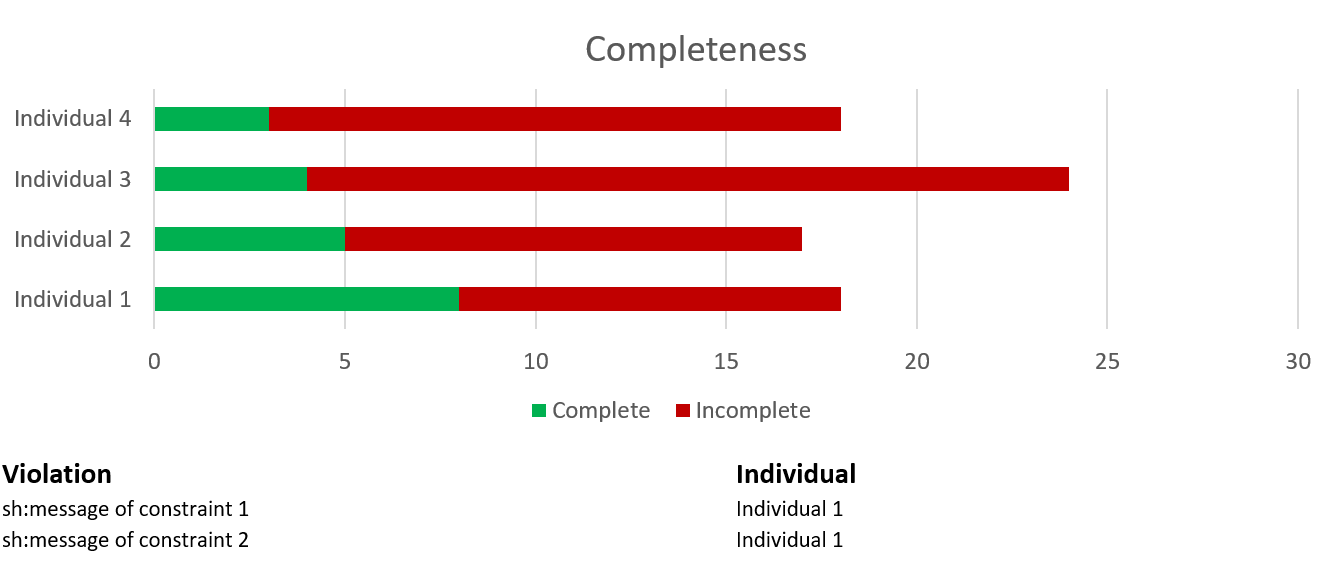
\includegraphics[width=16cm]{../../Images/04_Contribution/04_DecisionPresentationPattern_Component3_Example_Completeness.png}
  \caption{A mock-up of the presentation of the completeness maturity-level of four individuals. We show the completeness maturity-level for each individual using a bar chart.}
  \label{fig:Dashboard_Component_3_Completeness}
\end{figure} 

We extract the actual individual violations from the ontology. The $mvi_1$, $mvi_2$, $mvi_3$, and $mvi_4$ functions define the maximum number of violations per individual. We subtract the actual violations $av$ from the maximum violations $mv$ to get the information without conflict, the complete information, the reproducible information, and the aligned information.

\paragraph{Evidence spread dashboard}
The presentation of the evidence spread is a bit different. Instead of two data series, we need four data series: one for each evidence type. Figure \ref{fig:Dashboard_Component_3_Spread} presents an example of the presentation of the evidence spread of four individuals. We have chosen for a consistent colouring scheme, considering figure \ref{fig:Dashboard_Component_1}. We present the evidence spread for each individual using a bar chart. There are no constraints that enforce a specific evidence spread. Therefore, there are no violations to present. Instead, we present a list of evidence related to the selected individual below the bar chart. Furthermore, we consolidate the list of violations based on the root individuals. This presentation allows a decision-maker to understand the evidence spread and actual evidence related to a root individual. 

\begin{figure}[H]
\centering
  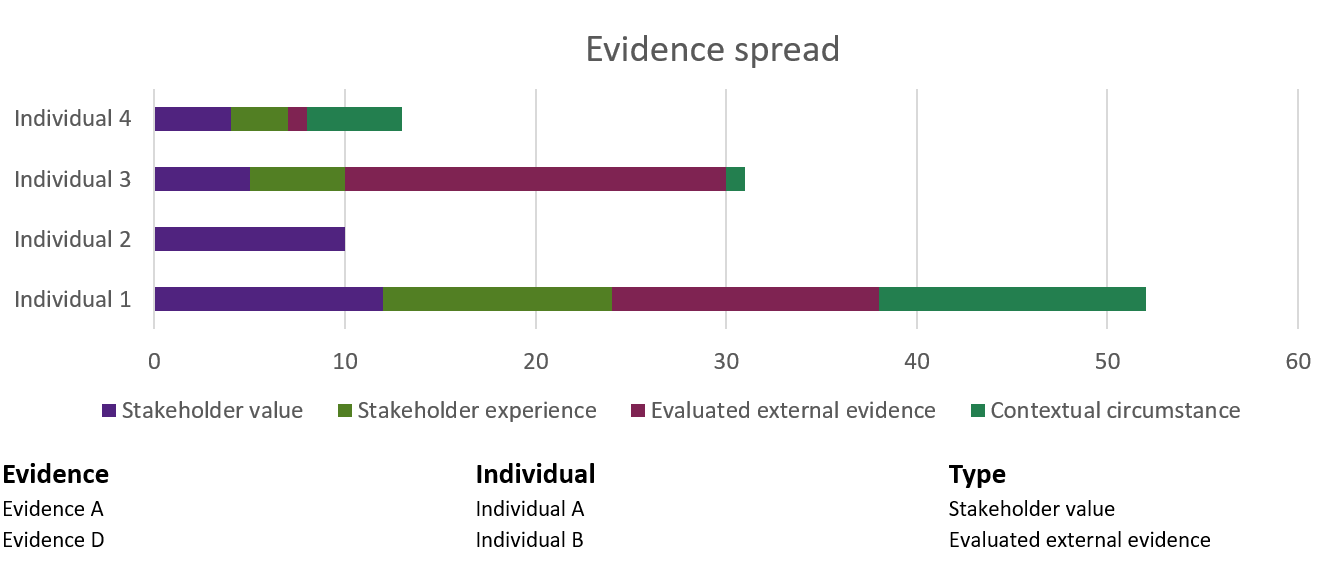
\includegraphics[width=16cm]{../../Images/04_Contribution/04_DecisionPresentationPattern_Component3_Example_Spread.png}
  \caption{A mock-up example of the presentation of the evidence spread of four individuals. We have chosen for a consistent colouring scheme, considering figure \ref{fig:Dashboard_Component_1}. We present the evidence spread for each individual using a bar chart.}
  \label{fig:Dashboard_Component_3_Spread}
\end{figure} 

We considered using an alternative presentation based on graphs. Figure \ref{fig:Dashboard_Component_3_Alternative} presents an example of this presentation. The graph-based presentation overwhelms the decision-maker with a lot of details, including the relationships between decision-relevant information and their status. This example presents only seven decision-relevant individuals. A more extensive example increases the size and complexity of the presentation. Additionally, the edges do not add useful information for the decision-maker.

\begin{figure}[H]
\centering
  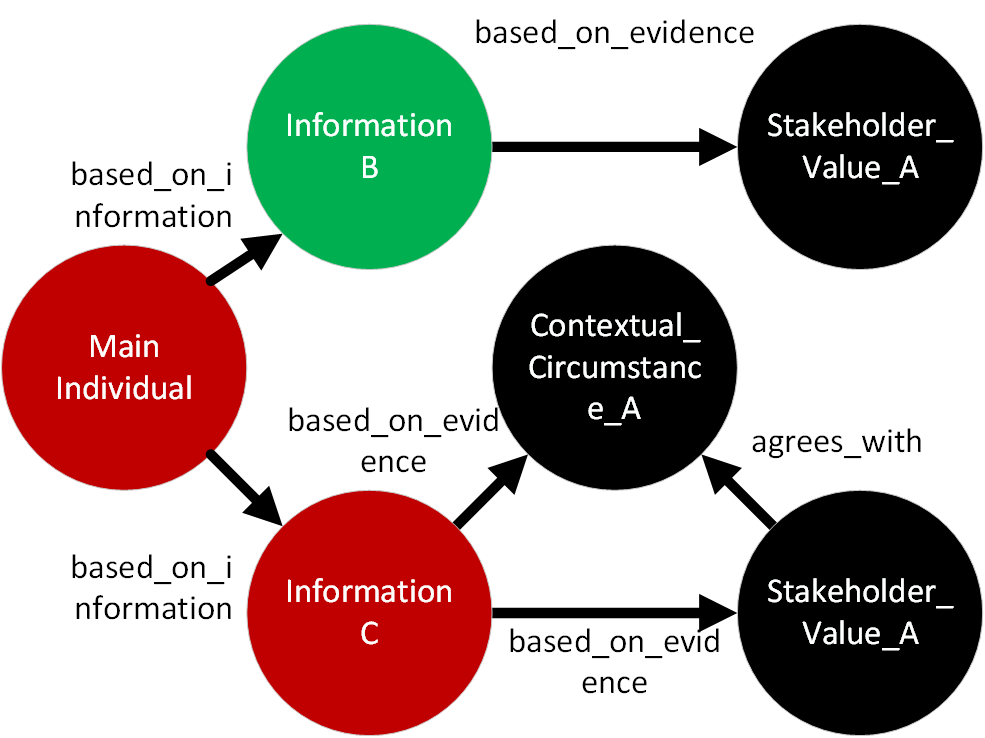
\includegraphics[width=7cm]{../../Images/04_Contribution/04_DecisionPresentationPattern_Component3_Example_Alternative.png}
  \caption{An alternative, more complex, presentation of the decision-relevant individuals and their maturity status.}
  \label{fig:Dashboard_Component_3_Alternative}
\end{figure} 
